\documentclass[notes,11pt, aspectratio=169]{beamer}

\usepackage{pgfpages}

\usepackage{helvet}
\usepackage[default]{lato}
\usepackage{array}
\usepackage{tikz}
\usepackage{verbatim}
\usepackage{stackengine}
\setbeamertemplate{note page}{\pagecolor{yellow!5}\insertnote}
\usetikzlibrary{positioning}
\usetikzlibrary{decorations}
\usetikzlibrary{calc}
\usetikzlibrary{arrows}
\usetikzlibrary{decorations.markings}
\usetikzlibrary{shapes.misc}
\usetikzlibrary{matrix,shapes,arrows,fit,tikzmark}
\usepackage{amsmath}
\usepackage{mathpazo}
\usepackage{hyperref}
\usepackage{lipsum}
\usepackage{multimedia}
\usepackage{graphicx}
\usepackage{multirow}
\usepackage{graphicx}
\usepackage{dcolumn}
\usepackage{bbm}
\usepackage{appendixnumberbeamer}
\newcolumntype{d}[0]{D{.}{.}{5}}

\graphicspath{ {./figures/} }

\usepackage{changepage}
\usepackage{appendixnumberbeamer}



\usepackage{graphicx}
\usepackage[space]{grffile}
\usepackage{booktabs}

% These are my colors -- there are many like them, but these ones are mine.
\definecolor{blue}{RGB}{0,114,178}
\definecolor{red}{RGB}{213,94,0}
\definecolor{yellow}{RGB}{240,228,66}
\definecolor{green}{RGB}{0,158,115}

\hypersetup{
  colorlinks=true,
  linkbordercolor = {white},
  linkcolor = {blue},
  urlcolor= {blue}
}


%% I use a beige off white for my background
\definecolor{MyBackground}{RGB}{255,253,218}

%% Uncomment this if you want to change the background color to something else
%\setbeamercolor{background canvas}{bg=MyBackground}

%% Change the bg color to adjust your transition slide background color!
\newenvironment{transitionframe}{
  \setbeamercolor{background canvas}{bg=yellow}
  \begin{frame}}{
    \end{frame}
}

\DeclareMathOperator*{\argmin}{arg\,min} 
\DeclareMathOperator*{\Var}{var}

\setbeamercolor{frametitle}{fg=blue}
\setbeamercolor{title}{fg=black}
\setbeamertemplate{footline}[frame number]
\setbeamertemplate{navigation symbols}{} 
\setbeamertemplate{itemize items}{-}
\setbeamercolor{itemize item}{fg=blue}
\setbeamercolor{itemize subitem}{fg=blue}
\setbeamercolor{enumerate item}{fg=blue}
\setbeamercolor{enumerate subitem}{fg=blue}
\setbeamercolor{button}{bg=MyBackground,fg=blue,}



% If you like road maps, rather than having clutter at the top, have a roadmap show up at the end of each section 
% (and after your introduction)
% Uncomment this is if you want the roadmap!
\AtBeginSection[]
{
  \begin{frame}
   \frametitle{Today's Presentation}
      \tableofcontents[currentsection]
  \end{frame}
}
\setbeamercolor{section in toc}{fg=blue}
\setbeamercolor{subsection in toc}{fg=red}
\setbeamersize{text margin left=1em,text margin right=1em} 

\newenvironment{wideitemize}{\itemize\addtolength{\itemsep}{10pt}}{\enditemize}

\usepackage{environ}
\NewEnviron{videoframe}[1]{
  \begin{frame}
    \vspace{-8pt}
    \begin{columns}[onlytextwidth, T] % align columns
      \begin{column}{.58\textwidth}
        \begin{minipage}[t][\textheight][t]
          {\dimexpr\textwidth}
          \vspace{8pt}
          \hspace{4pt} {\Large \sc \textcolor{blue}{#1}}
          \vspace{8pt}
          
          \BODY
        \end{minipage}
      \end{column}%
      \hfill%
      \begin{column}{.42\textwidth}
        \colorbox{green!20}{\begin{minipage}[t][1.2\textheight][t]
            {\dimexpr\textwidth}
            Face goes here
          \end{minipage}}
      \end{column}%
    \end{columns}
  \end{frame}
}

\title[]{\textcolor{blue}{Open School Enrollment and Residential Sorting}}
\author[MCC]{}
\institute[Yale]{\small{\begin{tabular}{c}
Crossan Cooper  \\
Yale University \\
\end{tabular}}}

\date{\today}


\begin{document}

%%% TIKZ STUFF
\tikzset{   
        every picture/.style={remember picture,baseline},
        every node/.style={anchor=base,align=center,outer sep=1.5pt},
        every path/.style={thick},
        }
\newcommand\marktopleft[1]{%
    \tikz[overlay,remember picture] 
        \node (marker-#1-a) at (-.3em,.3em) {};%
}
\newcommand\markbottomright[2]{%
    \tikz[overlay,remember picture] 
        \node (marker-#1-b) at (0em,0em) {};%
}
\tikzstyle{every picture}+=[remember picture] 
\tikzstyle{mybox} =[draw=black, very thick, rectangle, inner sep=10pt, inner ysep=20pt]
\tikzstyle{fancytitle} =[draw=black,fill=red, text=white]
%%%% END TIKZ STUFF

% Title Slide
\begin{frame}
\maketitle
\end{frame}

%\section{Introduction}

\begin{frame}{Overview}
\label{mapback}
  \begin{wideitemize}
    \item We know that where you live and where you go to school matter for both short- and long-run outcomes (Chetty et al. 2014, Altonji and Mansfield 2018)
    \item Neighborhood-based school assignment links the two
    \item In the last 30 years, explosion of school choice policies in the US seeking to improve \textcolor{red}{(a)} school quality, \textcolor{green}{(b)} access to high quality schools, or \textcolor{blue}{(c)} both \hyperlink{map}{\beamerbutton{Map}}
    \item \textbf{This project?} Explore how intradistrict open enrollment programs affect residential sorting within and across districts
    \begin{wideitemize}
    \item In the future, explore welfare consequences of policy adoption
    \end{wideitemize}
  \end{wideitemize}
  
\end{frame}



\begin{frame}{Literature}
\begin{wideitemize}
\item \textbf{Equilibrium residential sorting:} Tiebout 1956, Nechyba 2000, Epple and Romano 2003, Bayer et al. 2007, Ferreyra 2007, Avery and Pathak 2021
\item \textbf{Competitive effects of school choice:} Hoxby 2003, Rothstein 2006, MacLeod and Urquiola 2015, Barseghyan et al. 2019, Allende 2019, Neilson 2021, Campos and Kearns 2022
\begin{wideitemize}
    \item \textcolor{blue}{Hope to provide additional evidence for/against competitive effects of choice}
\end{wideitemize}
\item \textbf{Sorting responses to choice policies:} Reback 2005, Baum-Snow and Lutz 2011, Brunner et al. 2012, Altonji et al. 2015, Zheng 2022
\begin{wideitemize}
    \item \textcolor{blue}{No existing evidence on sorting responses to \textit{intradistrict} open enrollment}
\end{wideitemize}
\end{wideitemize}
\end{frame}

\begin{frame}{This Project}
\begin{alertblock}{Research Question 1: Housing Prices}
  What happens to the distribution of home prices after the switch from neighborhood assignment (NA) to open enrollment (OE)?
\end{alertblock}
\begin{exampleblock}{Research Question 2: Location}
  Do families relocate because of the policy? If so, are there differences in relocation patterns by family race or wealth level?
\end{exampleblock}
\begin{block}{Research Question 3: Welfare}
  What happens to household welfare after the introduction of open enrollment policies?
  % Which mechanism out of residential sorting and competitive incentives to improve school quality is stronger in equilibrium?
\end{block}
\medskip 
\begin{wideitemize}
    \item No evidence on \textcolor{red}{(1)} and \textcolor{green}{(2)} for intradistrict open enrollment policies
    \item Sign and magnitude of welfare changes in \textcolor{blue}{(3)} is ambiguous
\end{wideitemize}
\end{frame}

\section{Toy Model}

\begin{frame}{Big Picture} 
\label{detailsback}
\begin{wideitemize}
\item \textbf{Model Elements}
\begin{enumerate}
\item Households with type $x \in (0,1)$
\item A school district with 2 neighborhoods
\item One school in each neighborhood
\item Neighborhood home prices that only depend on school quality
\item Continuum of schools outside the district
\item Moving costs for leaving the district
\item $D(x)$ - a household's utility from staying in the district
\item $O(x)$ - a household's utility from leaving the district
\end{enumerate}
\item Assume that household preferences depend $\textcolor{green}{\uparrow}$ on school quality ($\textcolor{green}{\uparrow}$ in type), $\textcolor{red}{\downarrow}$ on home prices, and $\textcolor{green}{\uparrow}$ on living in the district
\item \textit{How do household preferences interact with school choice policy environment?}
\end{wideitemize}
\hyperlink{details}{\beamerbutton{Model Details}} \hyperlink{location}{\beamerbutton{Location Decision}} \hyperlink{example}{\beamerbutton{Numerical Example}}
\end{frame}

% \begin{frame}{Simple Numerical Example}
% \begin{wideitemize}
% \item Suppose $x \sim U(0,1)$ and $v(x,q) = x\cdot q$. The latter implies $p(q) = \frac{q^2}{2}$
% \item With this functional form, household of type $x$ will exit the district whenever
% \begin{equation*}
% O(x) = x\cdot x - \frac{x^2}{2} - \textcolor{red}{C}  >   x \cdot q_n - \frac{q_n^2}{2} = D(x)
% \end{equation*}
% \item This condition holds when
% \begin{equation*}
%  \frac{(x-q_n)^2}{2} > \textcolor{red}{C}
% \end{equation*}
% for both $n=1$ and $n=2$. Recall, higher $\textcolor{red}{C} \iff $ higher moving cost
% \item \textbf{Intuition:} Household will pay the moving cost and exit the district if it can't find a school close enough to its \textit{ideal} level within the district
% \begin{wideitemize}
% \item \textcolor{blue}{How does this exit condition interact with school choice policy?}
% \end{wideitemize}
% \end{wideitemize}
% \end{frame}

\begin{frame}{Moving from Neighborhood Assignment to Open Enrollment}
\begin{figure}
    \begin{overprint}
    \onslide<1>\centering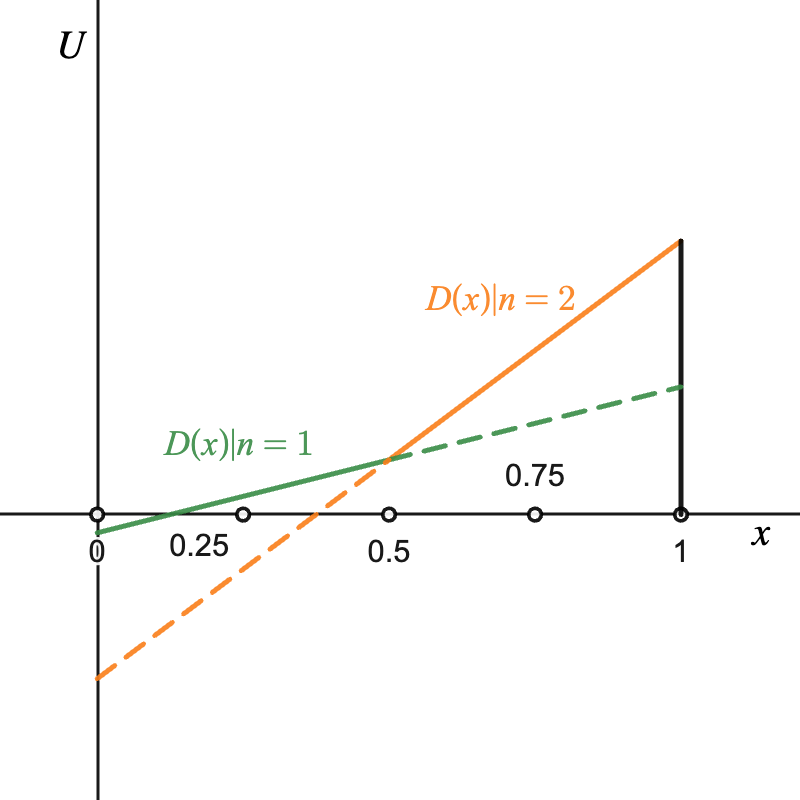
\includegraphics[width=0.4\textwidth]{figures/neighborhood_1.png}
    \caption{Symmetric neighborhood sorting equilibrium. Utility for marginal household of type $x$}
    \onslide<2>\centering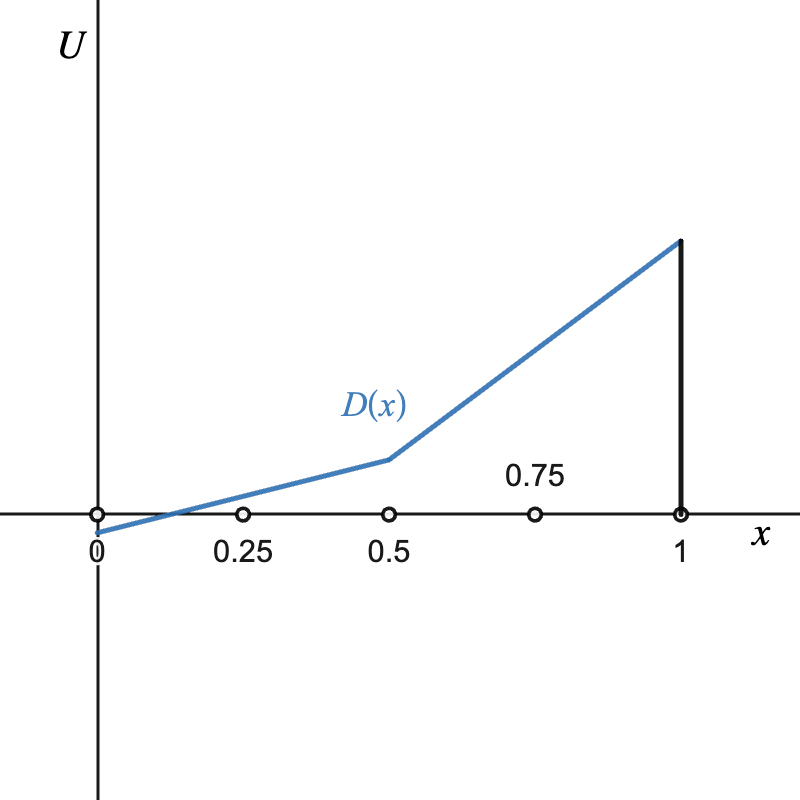
\includegraphics[width=0.4\textwidth]{figures/neighborhood_2.png}
    \caption{Level of utility in symmetric neighborhood sorting equilibrium}
    \onslide<3>\centering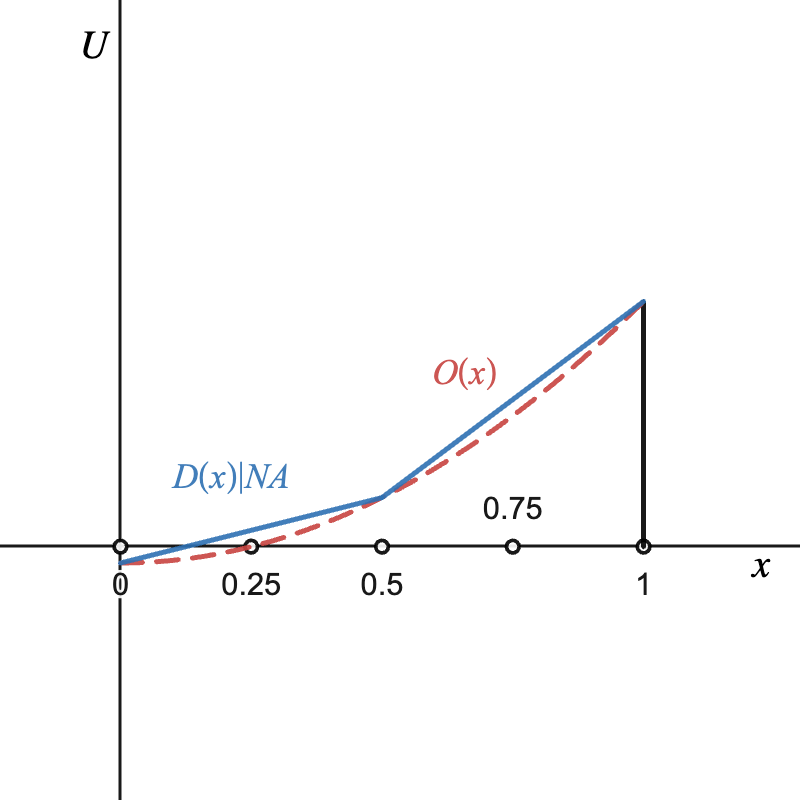
\includegraphics[width=0.4\textwidth]{figures/neighborhood.png}
    \caption{Lowest moving cost that results in no exit from neighborhood sorting equilibrium}
    \onslide<4>\centering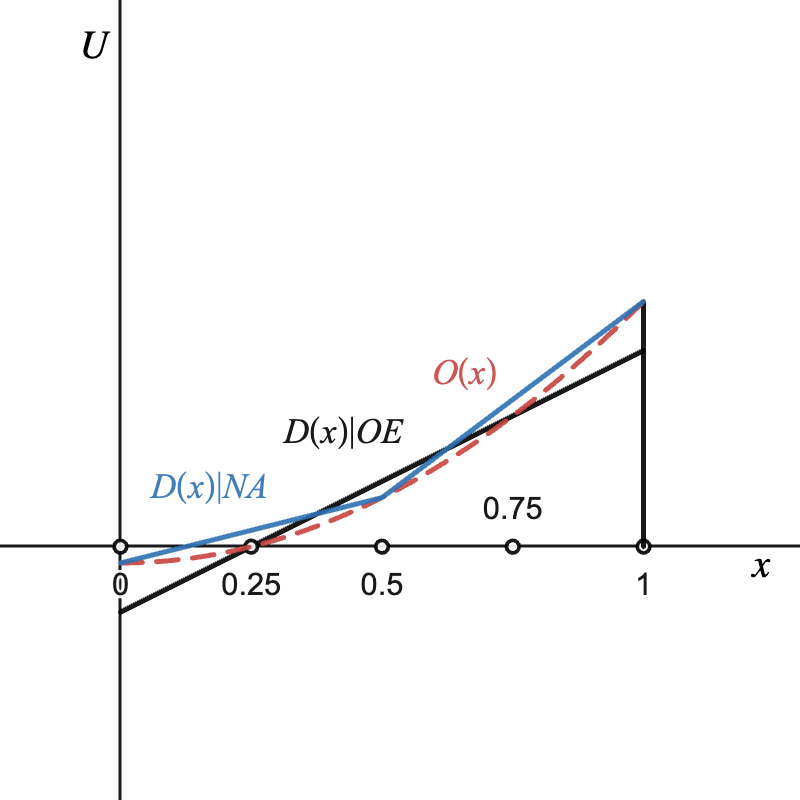
\includegraphics[width=0.4\textwidth]{figures/all.png}
    \caption{Open enrollment equalizes school quality. Utility levels change}
    \onslide<5>\centering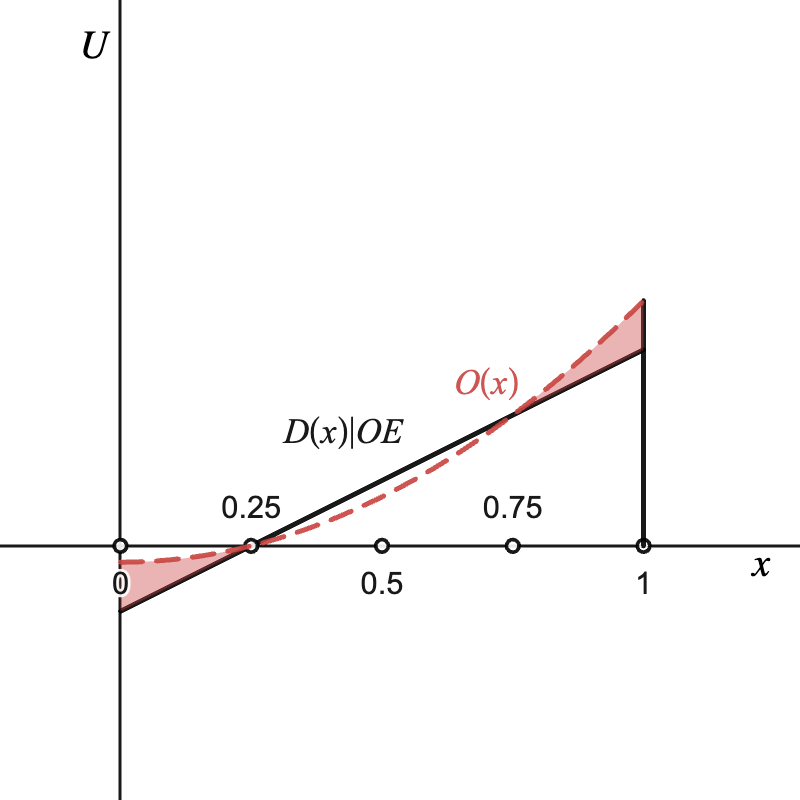
\includegraphics[width=0.4\textwidth]{figures/school_choice.png}
    \caption{Same set of options outside district $\implies$ households will exit from top and bottom}
    \end{overprint}
\end{figure}
\end{frame}

% \begin{frame}{When will everyone stay under School Choice?}
% \begin{figure}
% \centering
% 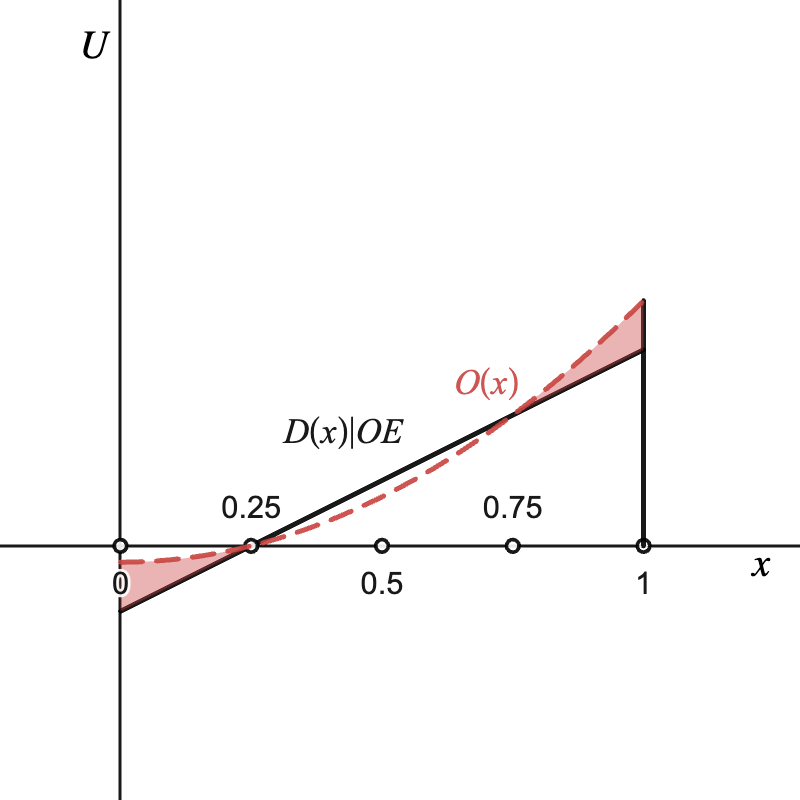
\includegraphics[width=0.75\textwidth]{figures/school_choice.png}
% \caption{School Choice Equilibrium with $x \sim U(0,1)$}
% \end{figure}
% \end{frame}

\begin{frame}{Toy Model Insights}
\label{databack}
\begin{wideitemize}
\item \textcolor{blue}{The key mechanism?} When school choice is introduced, school qualities equalize. Competitive housing market leads to
\begin{enumerate}
\item $\textcolor{green}{\uparrow}$ home prices in neighborhood with originally lower-quality school
\item $\textcolor{red}{\downarrow}$ home prices in neighborhood with originally higher-quality school
\end{enumerate}
\item High types exit due to $\textcolor{red}{\downarrow}$ in school quality, low types exit due to $\textcolor{green}{\uparrow}$ in home prices
\item Lots of reasons to think this pattern might not hold up in practice:
\begin{enumerate}
    \item Homes and neighborhoods are differentiated
    \item Schools do not adjust to the same quality under school choice because of exogenous fixed factors, frictions in the choice process
    \item Home prices are sticky, families may be immobile in their residential choices
\end{enumerate} 
\item Guided by toy model, want to explore $\Delta$ school quality and $\Delta$ home prices \hyperlink{data}{\beamerbutton{Data}}
\end{wideitemize}
\end{frame}

\section{Empirical Results}

\begin{frame}{Home Price Responses to Intradistrict Open Enrollment}
\label{giniback}
\begin{figure}
\centering
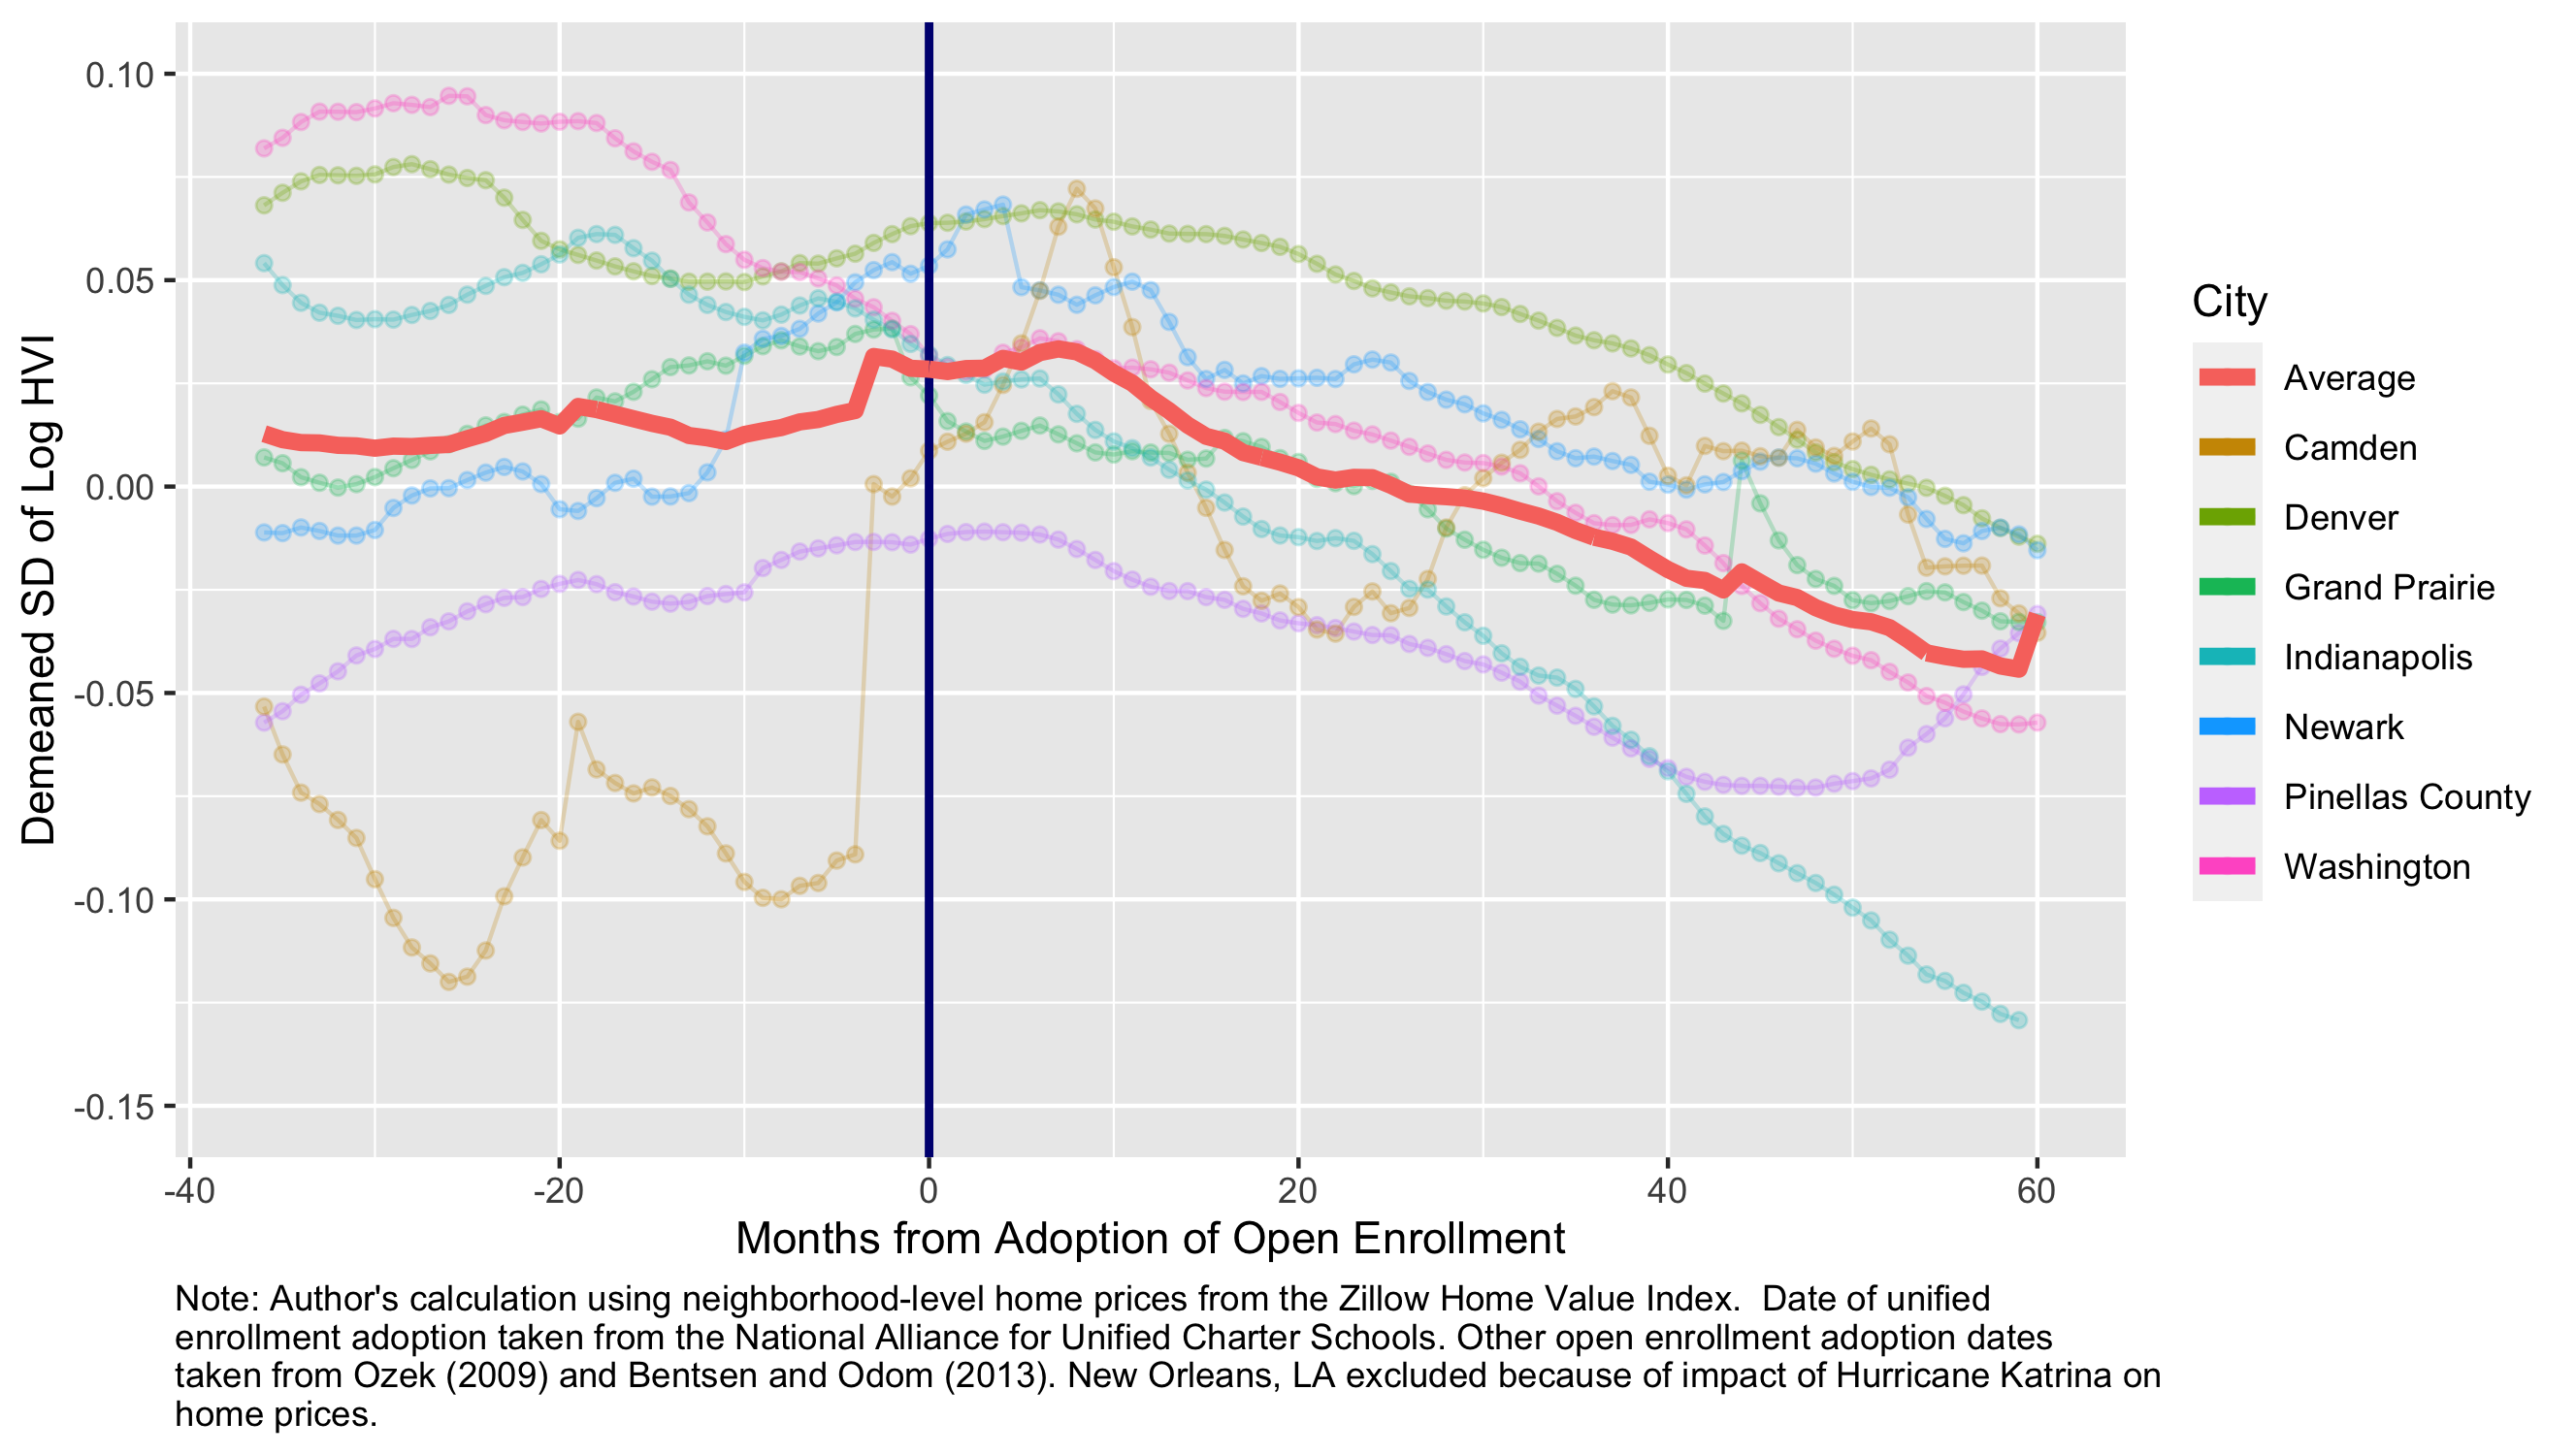
\includegraphics[width=0.8\textwidth]{figures/demeaned_hpi_sd_MONTHLY.png}
\end{figure}
\hyperlink{gini}{\beamerbutton{Gini Index}} \hyperlink{sumstats}{\beamerbutton{Summary Stats}}
\end{frame}

% \begin{frame}{School District Synthetic Controls Framework}
% % be explicit about treatment and control group
% \begin{wideitemize}
% \item Want to know how open enrollment impacts the distribution of home prices within a school district. But no clear control group
% \item \textbf{Potential solution?} Adopt augmented synthetic control method (Ben-Michael et al. 2021) to construct valid synthetic controls for treated districts and deal with staggered policy adoption
% \item \textit{Pool of potential control school districts:} 4418 districts in the top 25\% of student enrollment (above 2169 students)
% \item \textit{Matching strategy:} pre-treatment levels of \textcolor{blue}{(1)} outcome variable and \textcolor{blue}{(2)} per-student spending, \textcolor{blue}{(3)} student-teacher ratio, \textcolor{blue}{(4)} \% free and reduced price lunch, \textcolor{blue}{(5)} \% under-represented minority, \textcolor{blue}{(6)} number of schools, \textcolor{blue}{(7)} number of students
% % \item SE's are clustered at the district-year level
% % \item \textbf{Identifying Assumption:} without the open enrollment policy, the difference in district-level outcomes between observably similar districts is constant over time
% \end{wideitemize}
% \end{frame}

% \begin{frame}{School District Synthetic Controls Results}
% % figure of home price appreciation after the adoption date separately for high and low neighborhoods
% \end{frame}

\begin{frame}{District Diff-in-Diff Framework}
% be explicit about treatment and control group
\begin{wideitemize}
\item Consider a staggered DiD design at the school district-month (year) level\[Y_{dt} = \phi_d + \gamma_t + \sum_{k \ne -1 } \textcolor{purple}{\beta_k} \cdot \mathbf{1}\{\text{$k$ periods from OE}\}_{dt} + \mathbf{X}_{dt}^{'} \Gamma + \epsilon_{dt} \]
% need to think about where to cluster SE's
\item \textbf{Treatment Group:} 7 school districts adopting open enrollment since 2000
\item \textbf{Control Group:} districts in the same metro areas that do not adopt open enrollment
\item \textbf{Data:} Home prices from Zillow HVI, test scores from Educational Opportunity Project, district characteristics from NCES
% \item \textit{Predictions:} Gini index will fall in adopting districts relative to cities in the same metro area that do not adopt
\end{wideitemize}
\end{frame}

\begin{frame}{District Diff-in-Diff: SD of Log HVI (Mean = 0.39)}
\label{sd}
\begin{figure}
\centering
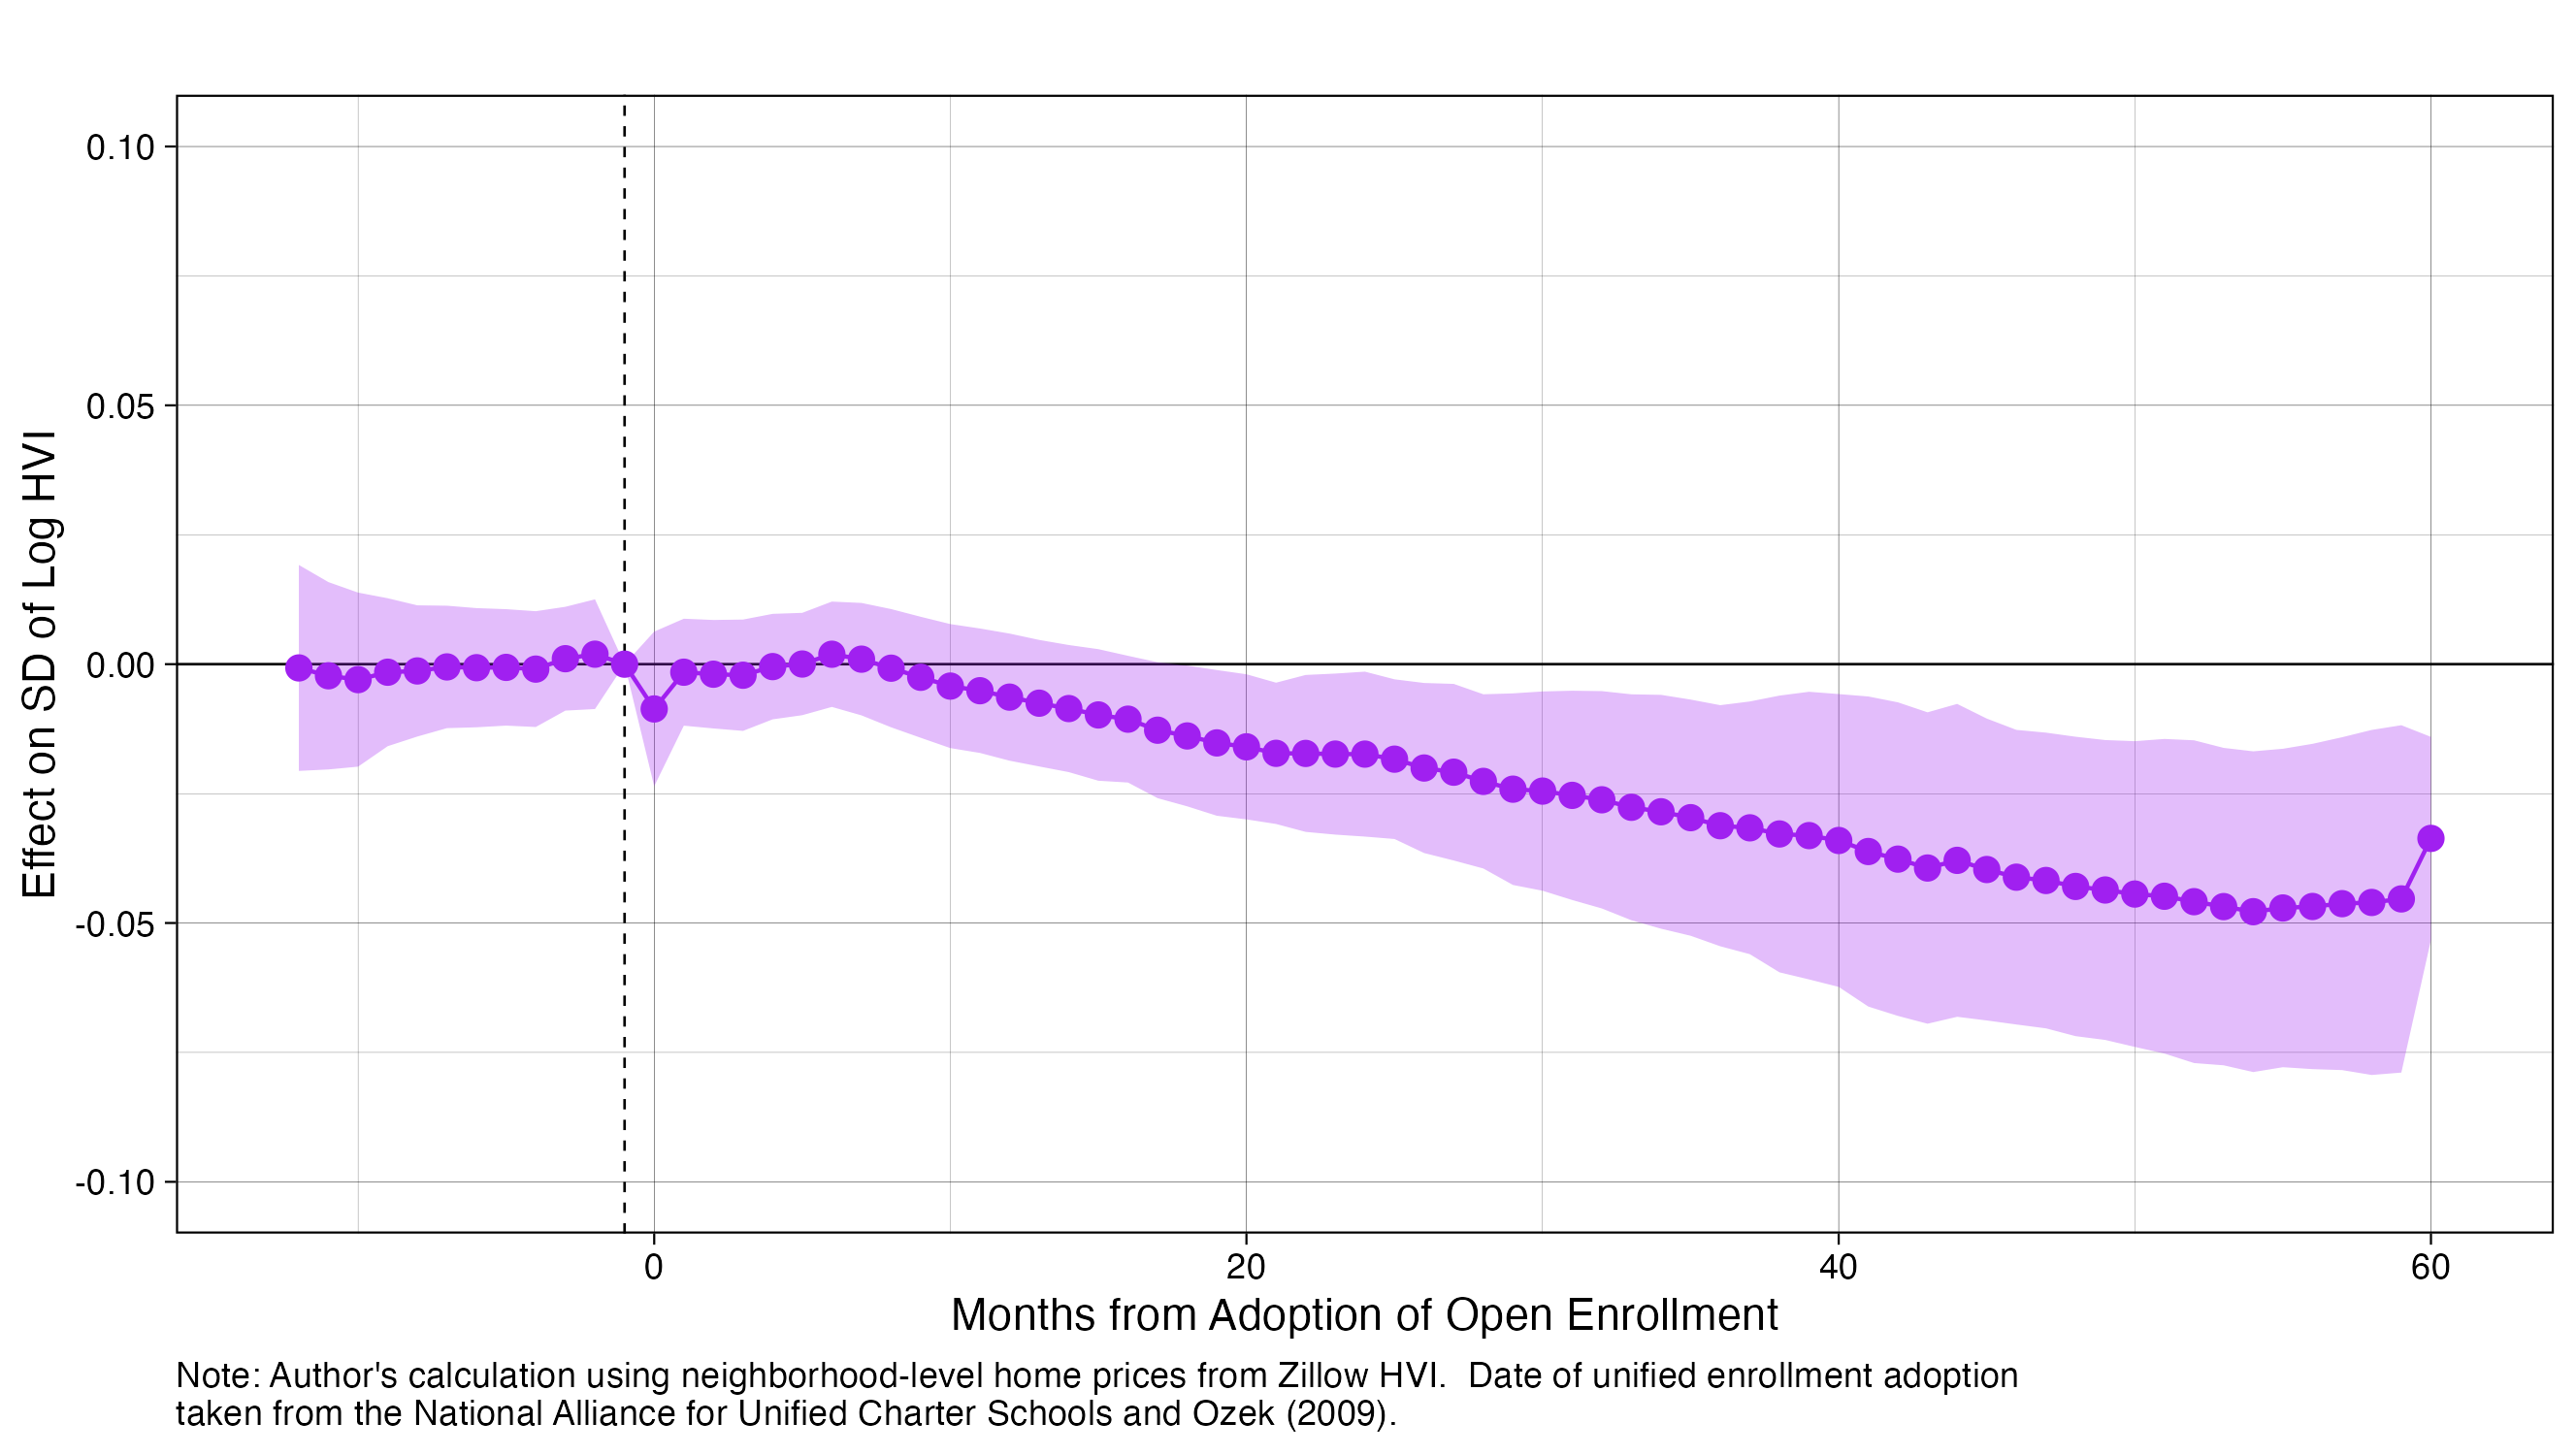
\includegraphics[width=0.8\textwidth]{figures/event_study_sd.png}
\end{figure}
\hyperlink{gini_did}{\beamerbutton{Gini Index}}
\end{frame}

\begin{frame}{District Diff-in-Diff: Average Test Scores}
\begin{figure}
\centering
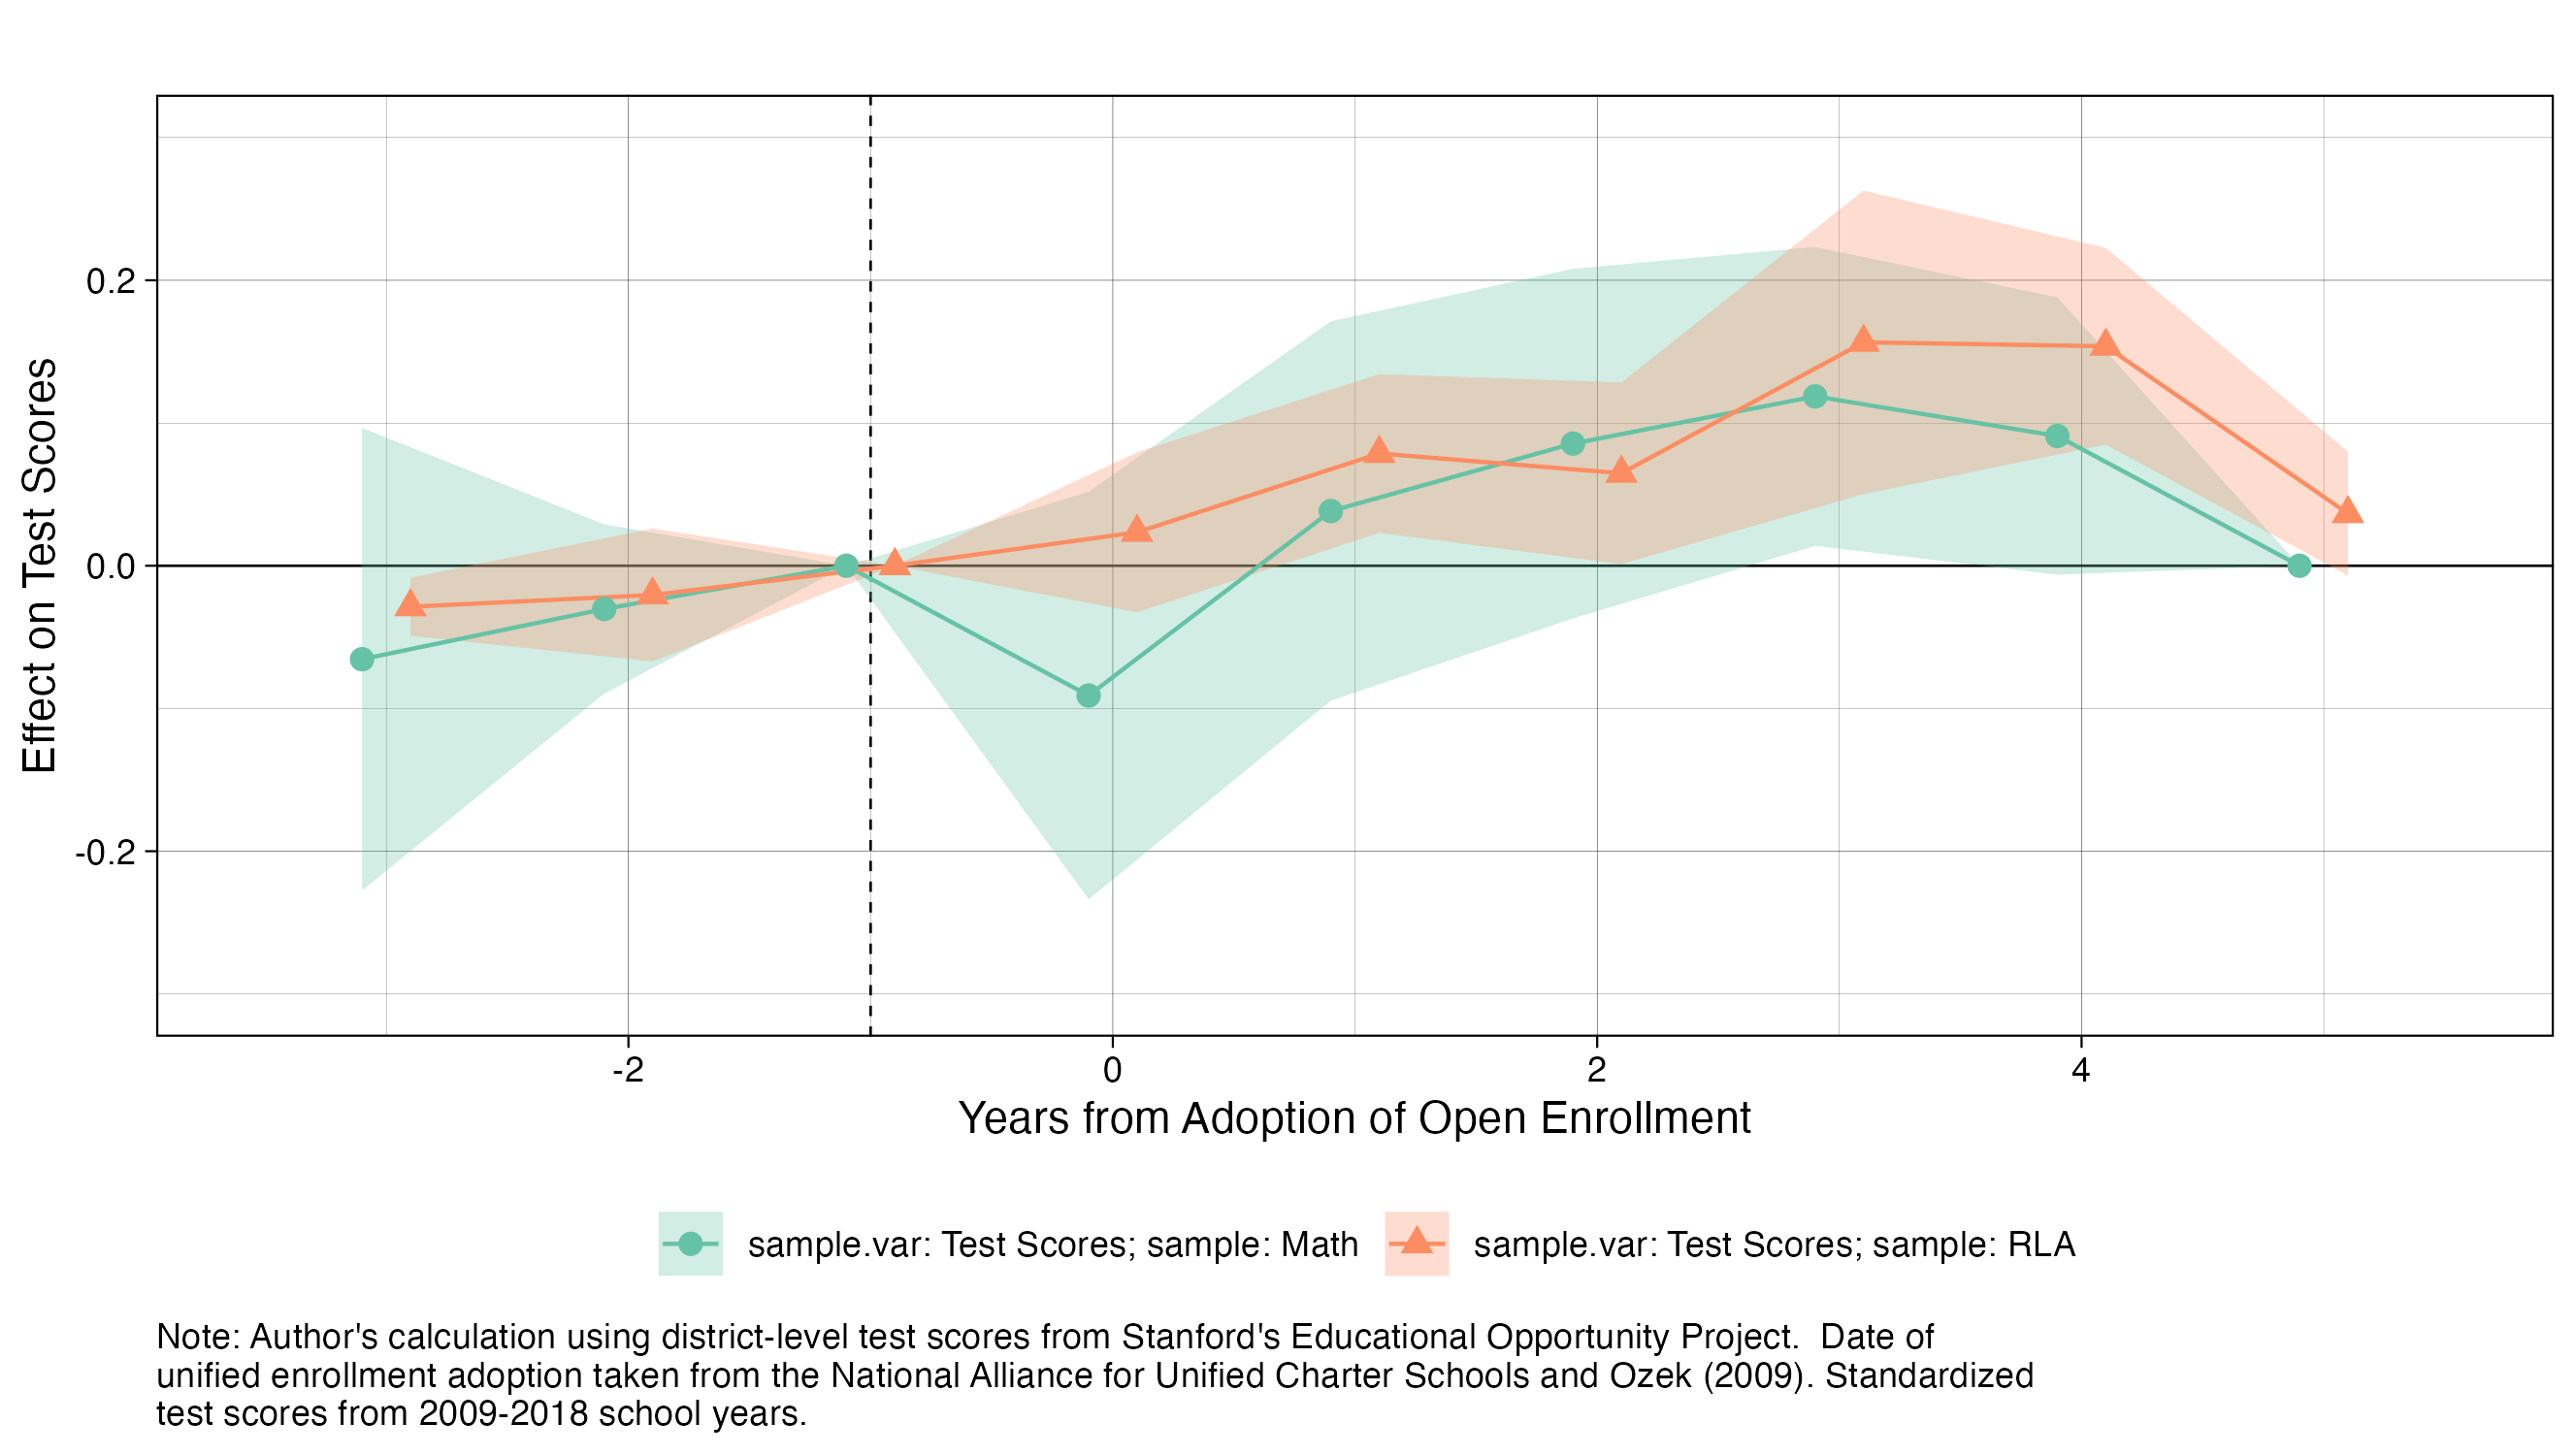
\includegraphics[width=0.8\textwidth]{figures/did_scores.png}
\end{figure}
\end{frame}

\begin{frame}{Neighborhood Event Study Framework}
% be explicit about treatment and control group
\begin{wideitemize}
\item Now consider a staggered event study design at the census tract-year level\[Y_{nt}^q = \phi_d + \gamma_t^q + \sum_{k \ne -1 } \textcolor{purple}{\beta_k^q} \cdot \mathbf{1}\{\text{$k$ years from OE}\}_{nt} +  \epsilon_{nt}^q \]
where $q$ indexes HH income quintiles across tracts within districts $d$
\item \textbf{Sample}: census tracts from 4 largest adopting districts matched with FHFA HPI tract-level home appreciation data (64-126 matched tracts per district)
\item \textcolor{purple}{Open Enrollment TE}: changes in home price appreciation due to open enrollment
\item \textit{Prediction:} appreciation should be higher for lower median HH income tracts
\end{wideitemize}
\end{frame}

\begin{frame}{Neighborhood Event Study: House Appreciation}
\begin{figure}
\centering
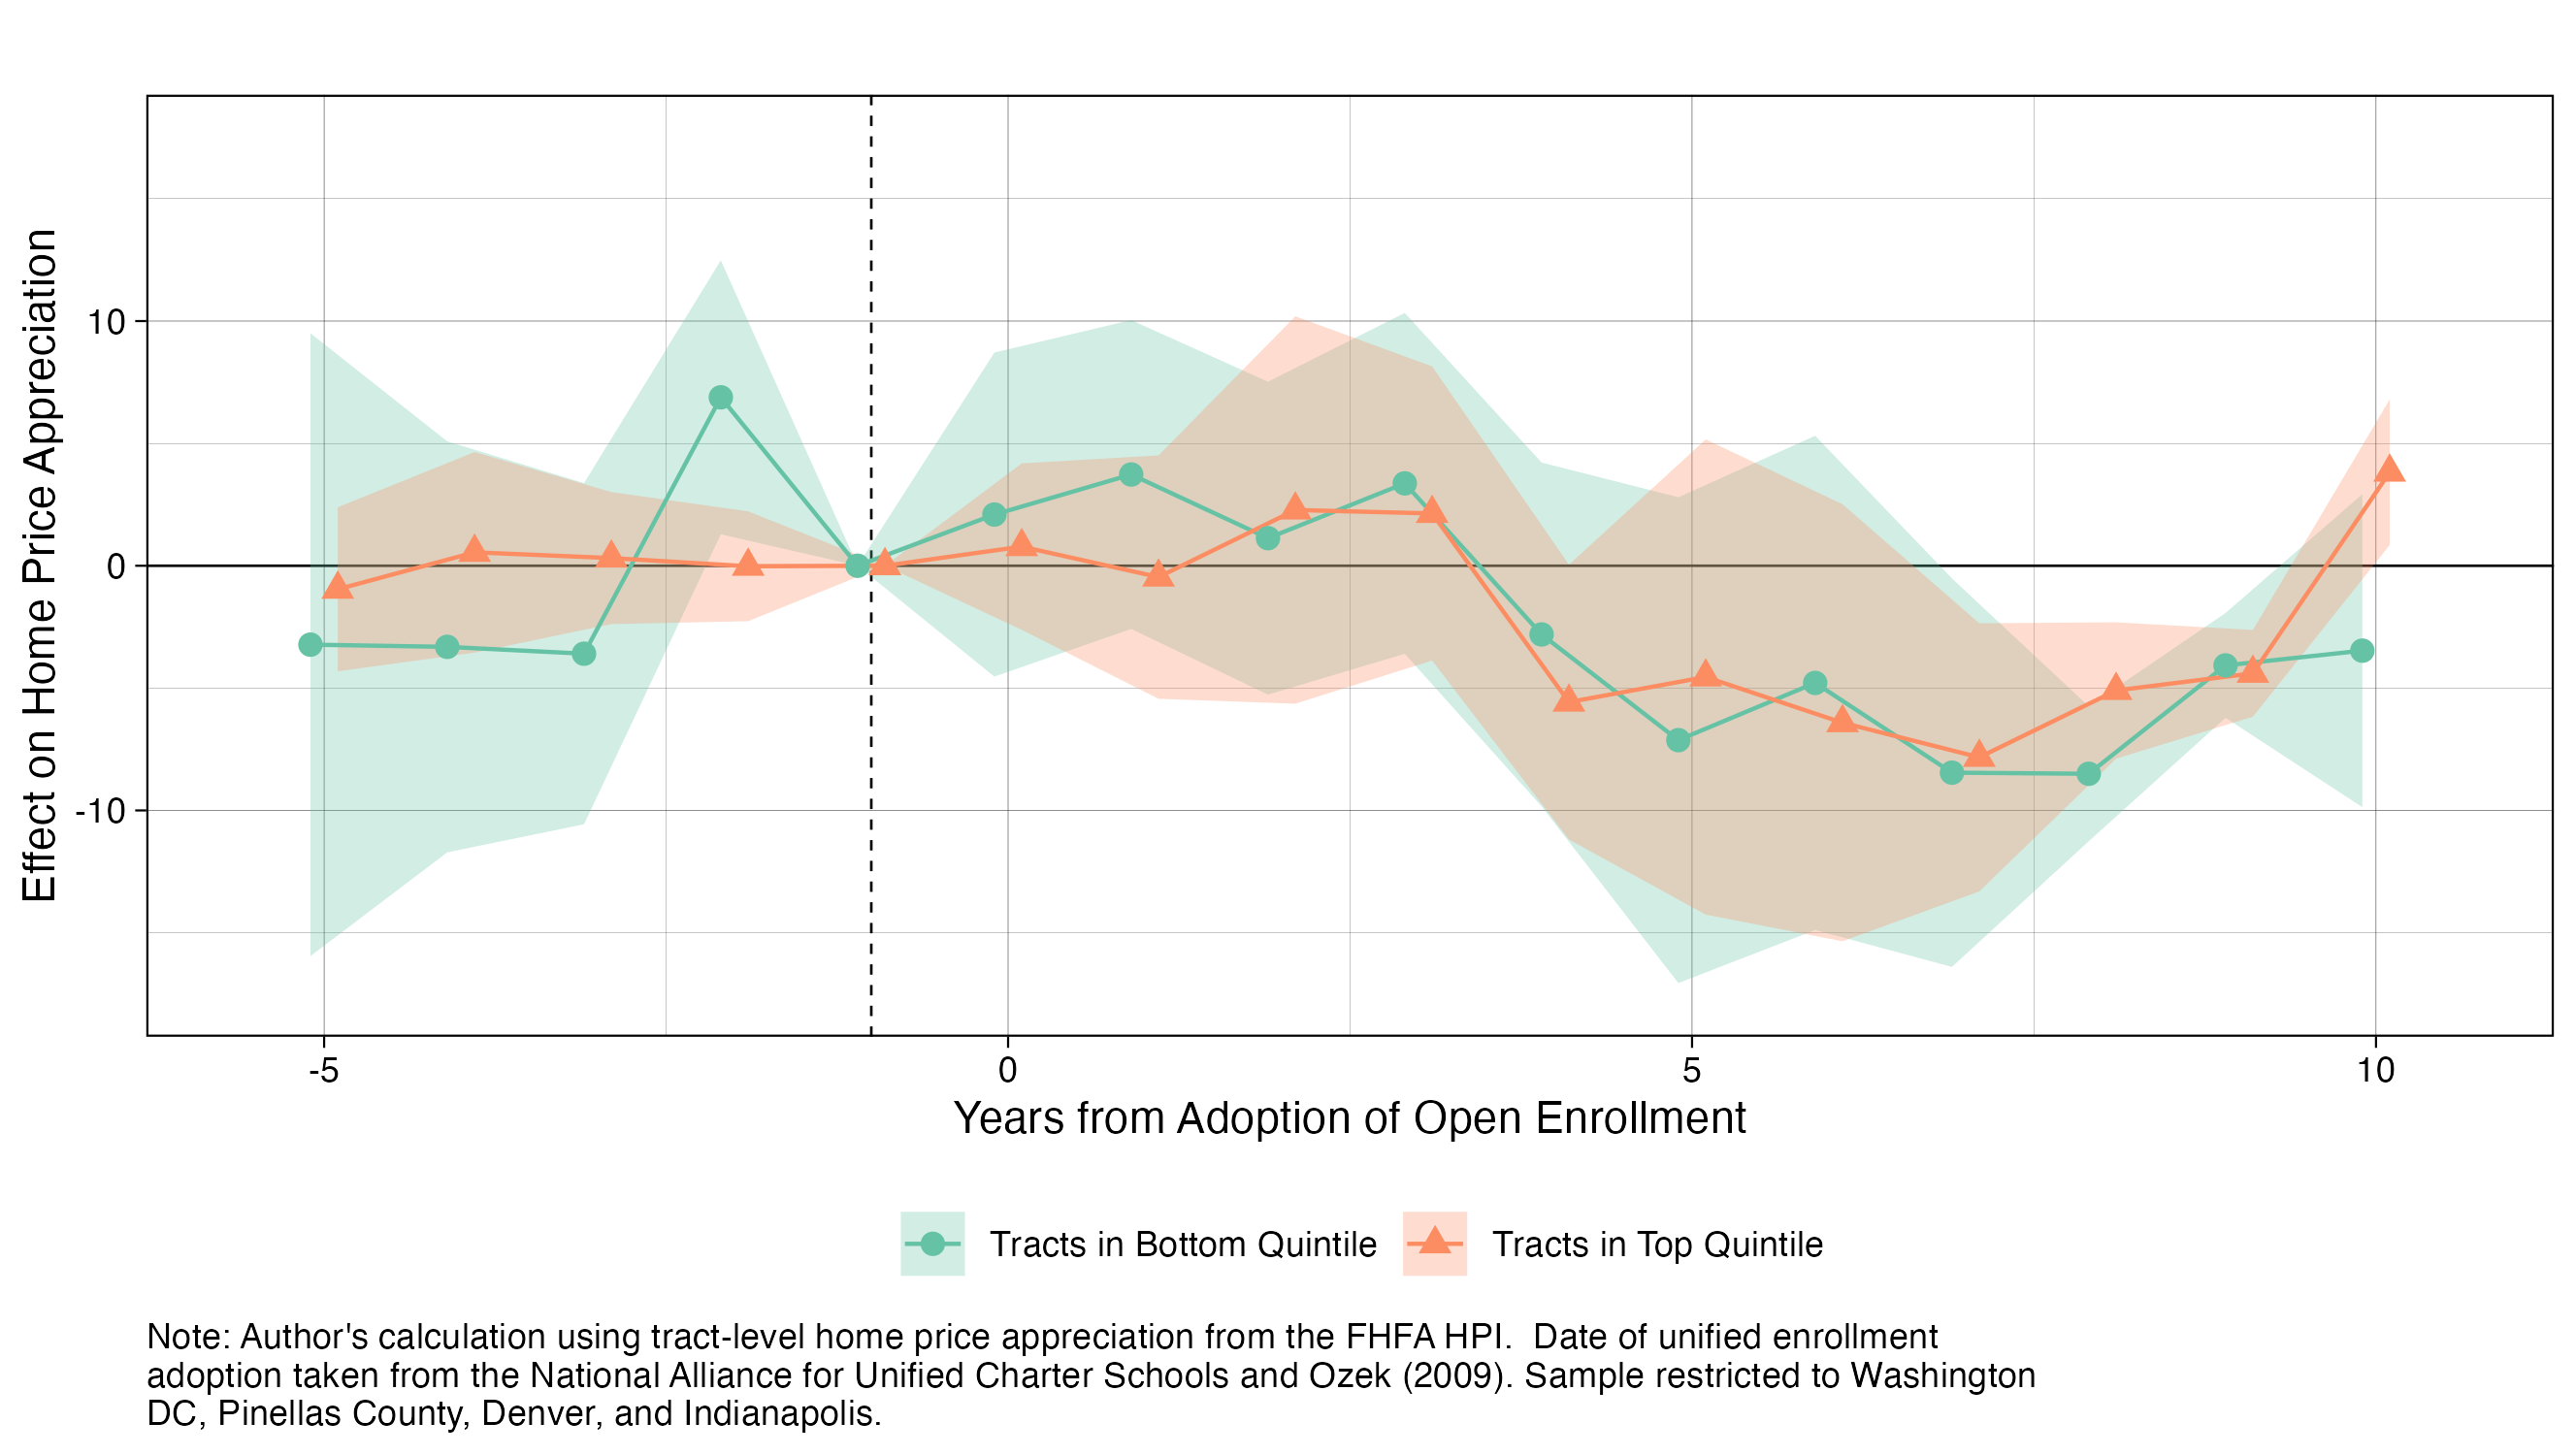
\includegraphics[width=0.9\textwidth]{figures/event_study_appreciation.png}
\end{figure}
\end{frame}

% \begin{frame}{Neighborhood Diff-in-Diff: Percent URM}

% \end{frame}

% \section{Descriptive Hedonics}

% \begin{frame}{Hedonics}
% \begin{wideitemize}
% \item Consider a hedonic model of neighborhood home prices %
% \[ \log p_{nt} = \textcolor{blue}{\beta_t} \mathbf{X}_{nt} + \epsilon_{nt} \] where %
% $\mathbf{X}_{nt}$ is a vector of neighborhood characteristics including neighborhood school quality, median household income, and average level of parental education
% \item What happens after a district moves from neighborhood assignment to open enrollment? In particular, how does $\textcolor{blue}{\beta_t^{school}}$ change? 
% \item Intuition from the school quality capitalization literature (e.g. Black 1999) suggests that $\textcolor{blue}{\beta_t^{school}}$ $\uparrow$ in catchment areas of low-performing schools and $\downarrow$ in catchment areas of high-performing schools
% \end{wideitemize}
% \end{frame}

% \begin{frame}{Hedonic Model Parameter Estimates}
% % make a table here
% \end{frame}

\section{Looking Ahead}

% \begin{frame}{Sketching a Model}
% \begin{wideitemize}
%     \item Want to adopt a sufficient statistics approach to estimate the equilibrium response to the school choice policy
% \end{wideitemize}
% \end{frame}

\begin{frame}{Conclusion}
\begin{wideitemize}
    \item \textbf{What did I show you today?}
    \begin{enumerate}
    \item A toy model highlighting two related mechanisms (i.e. \textcolor{red}{changes to home prices \& changes to school quality}) that might induce out-of-district migration after open enrollment
    \item Suggestive reduced-form evidence that the within-district distribution of home prices does respond to open enrollment policies
    \end{enumerate}
    \item \textbf{What is coming next?}
    \begin{enumerate}
    \item Additional reduced-form work using CoreLogic and school-level test score data
    \item Revisiting existing results after building crosswalk between SAB's and census tracts
    \item A richer model with vertical and horizontal differentiation to characterize sorting across neighborhoods and school districts
    \end{enumerate}
\end{wideitemize}
\end{frame}


\begin{frame}
  \centering \Huge
  %\emph{Thank You For Coming!}
  Thank You For Coming!

  \bigskip 
  \centering \small
  Questions or comments? \url{crossan.cooper@yale.edu}
\end{frame}

\section*{Extra Slides}

\appendix

\begin{frame}{Landscape of Open Enrollment in the US} 
% insert the map here
\label{map}
\centering
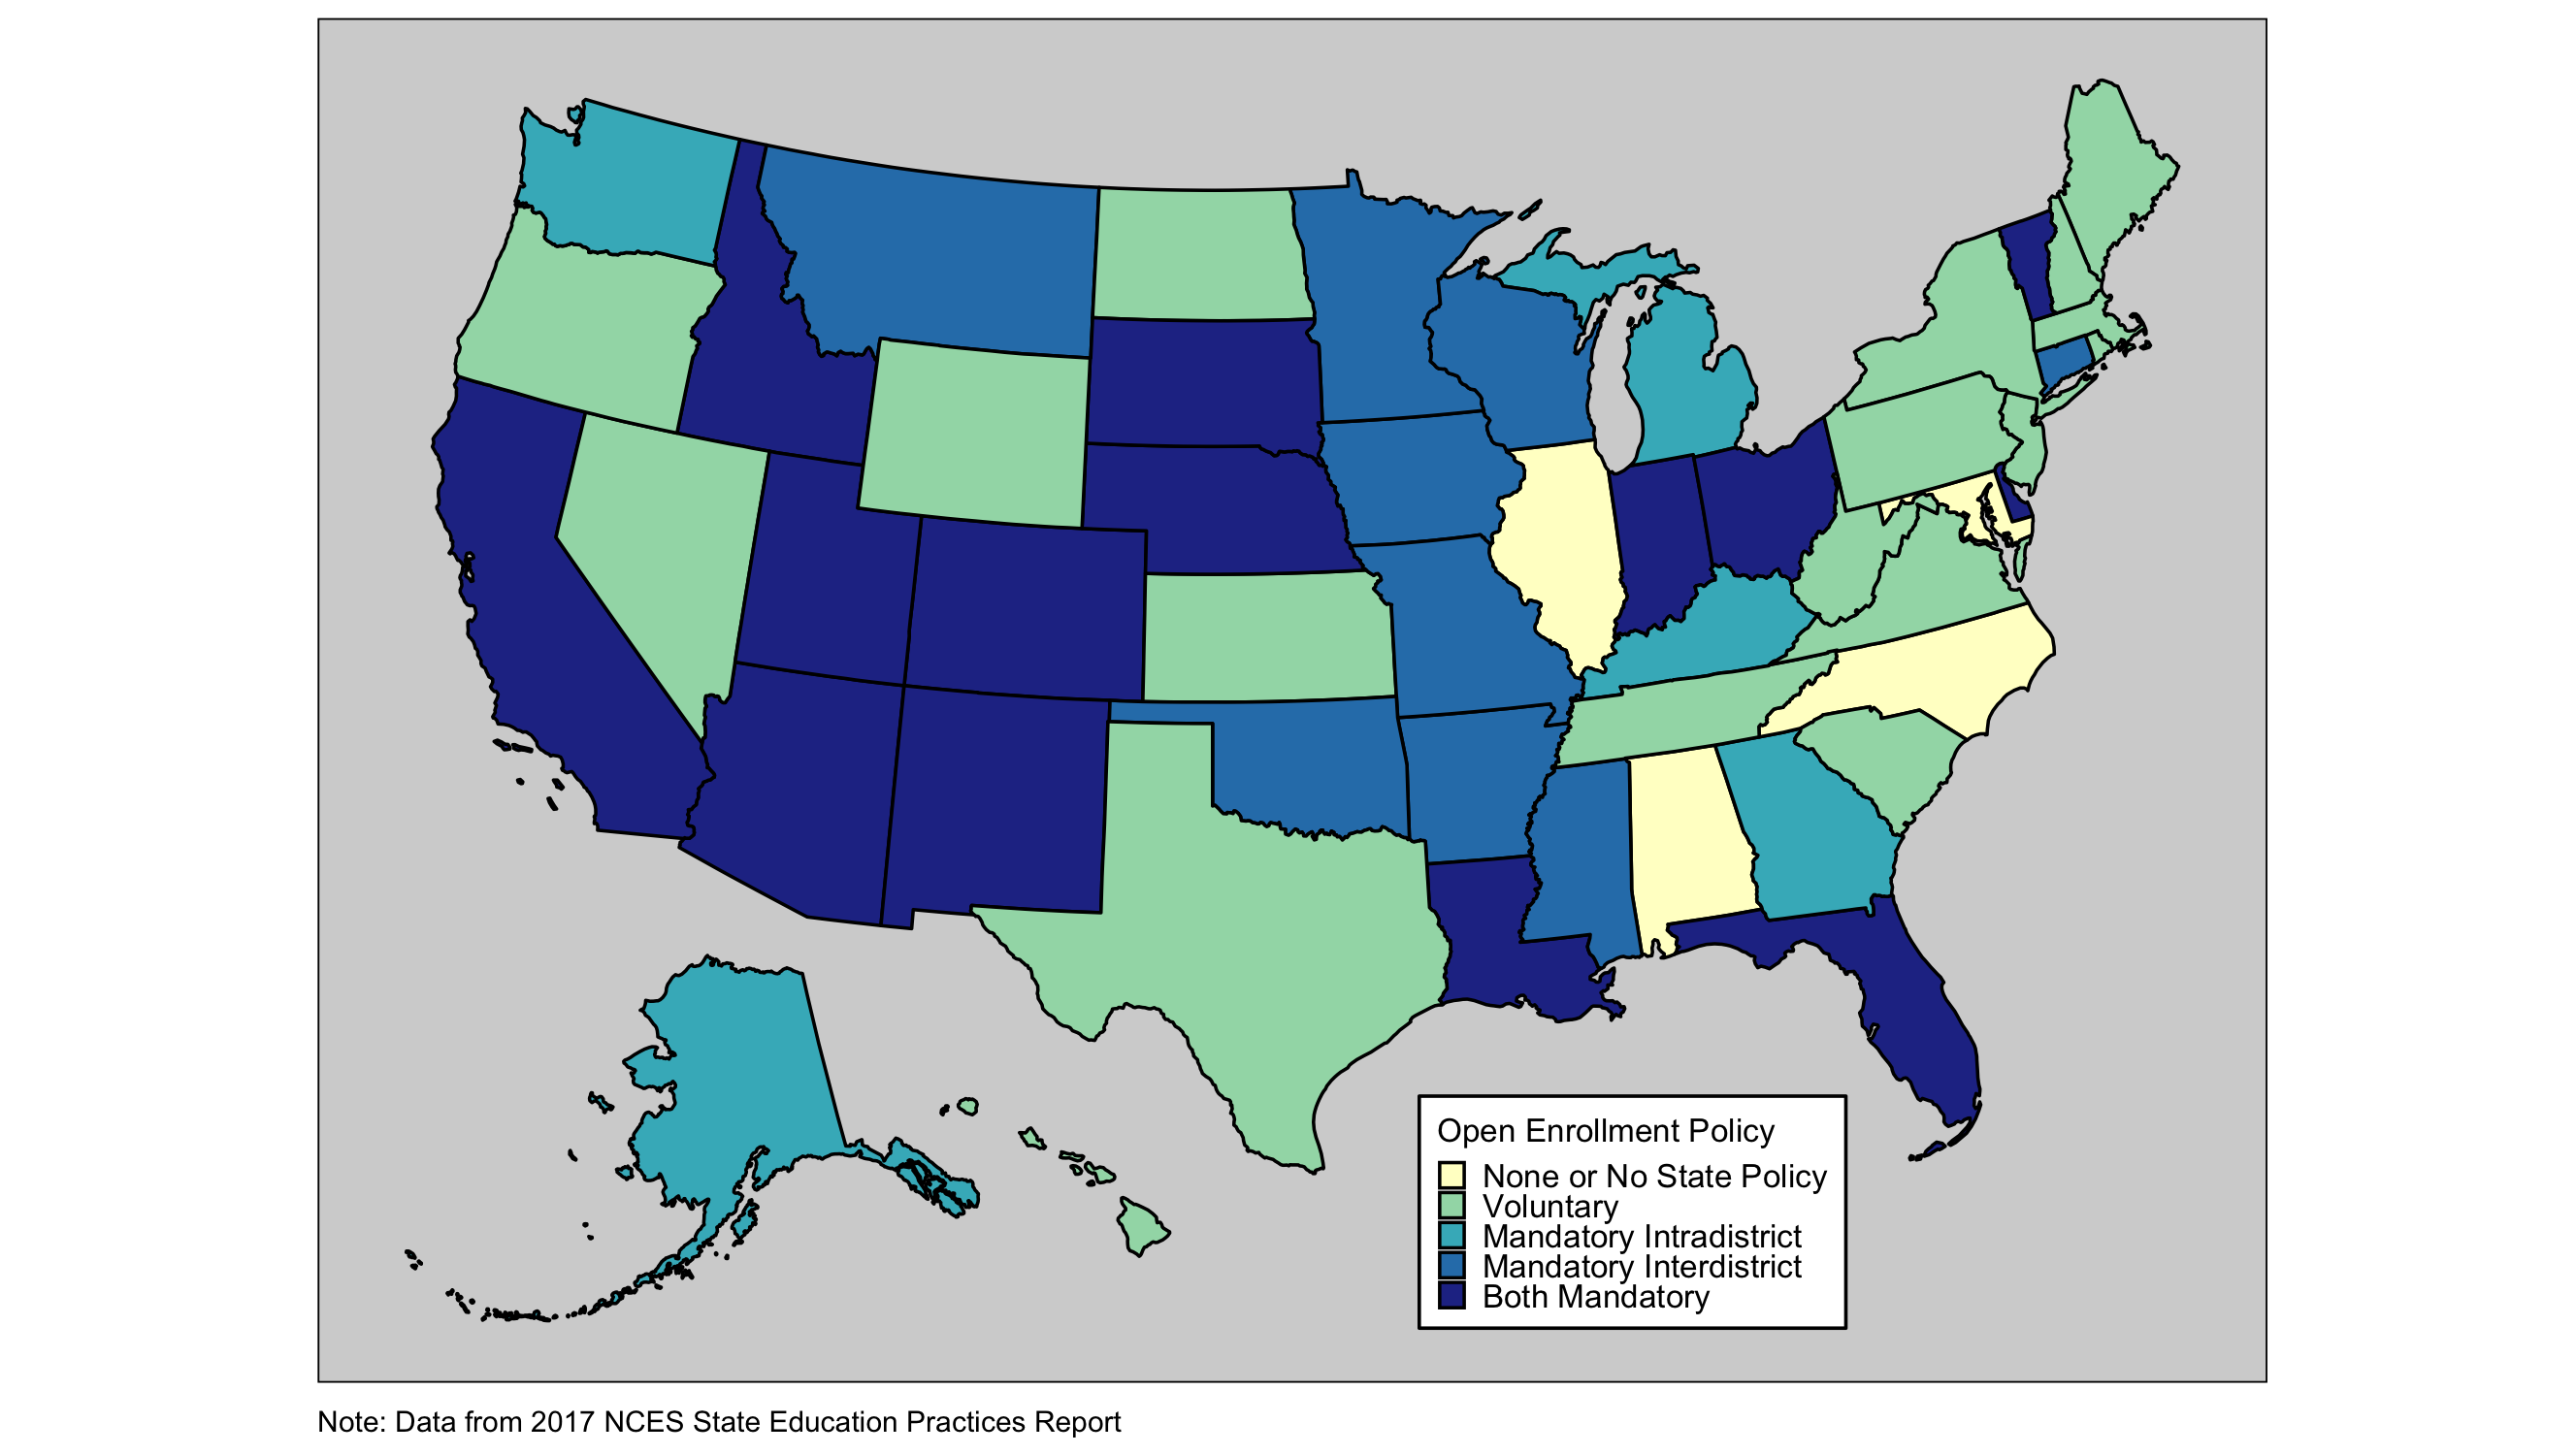
\includegraphics[width=0.8\textwidth]{figures/policies_map.png}
  \begin{wideitemize}
    \item Open enrollment plans began in the US in 1988 and are still being debated: Kansas just passed open enrollment legislation for the 2024-2025 school year \hyperlink{mapback}{\beamerbutton{Back}}
    %\item Practitioners and policy-makers distinguish between \textcolor{red}{voluntary} and \textcolor{red}{mandatory} open enrollment as well as \textcolor{green}{intradistrict} versus \textcolor{green}{interdistrict} transfer policies
  \end{wideitemize}
  
\end{frame}

\begin{frame}{Home Price Responses to Intradistrict Open Enrollment}
\label{gini}
\centering
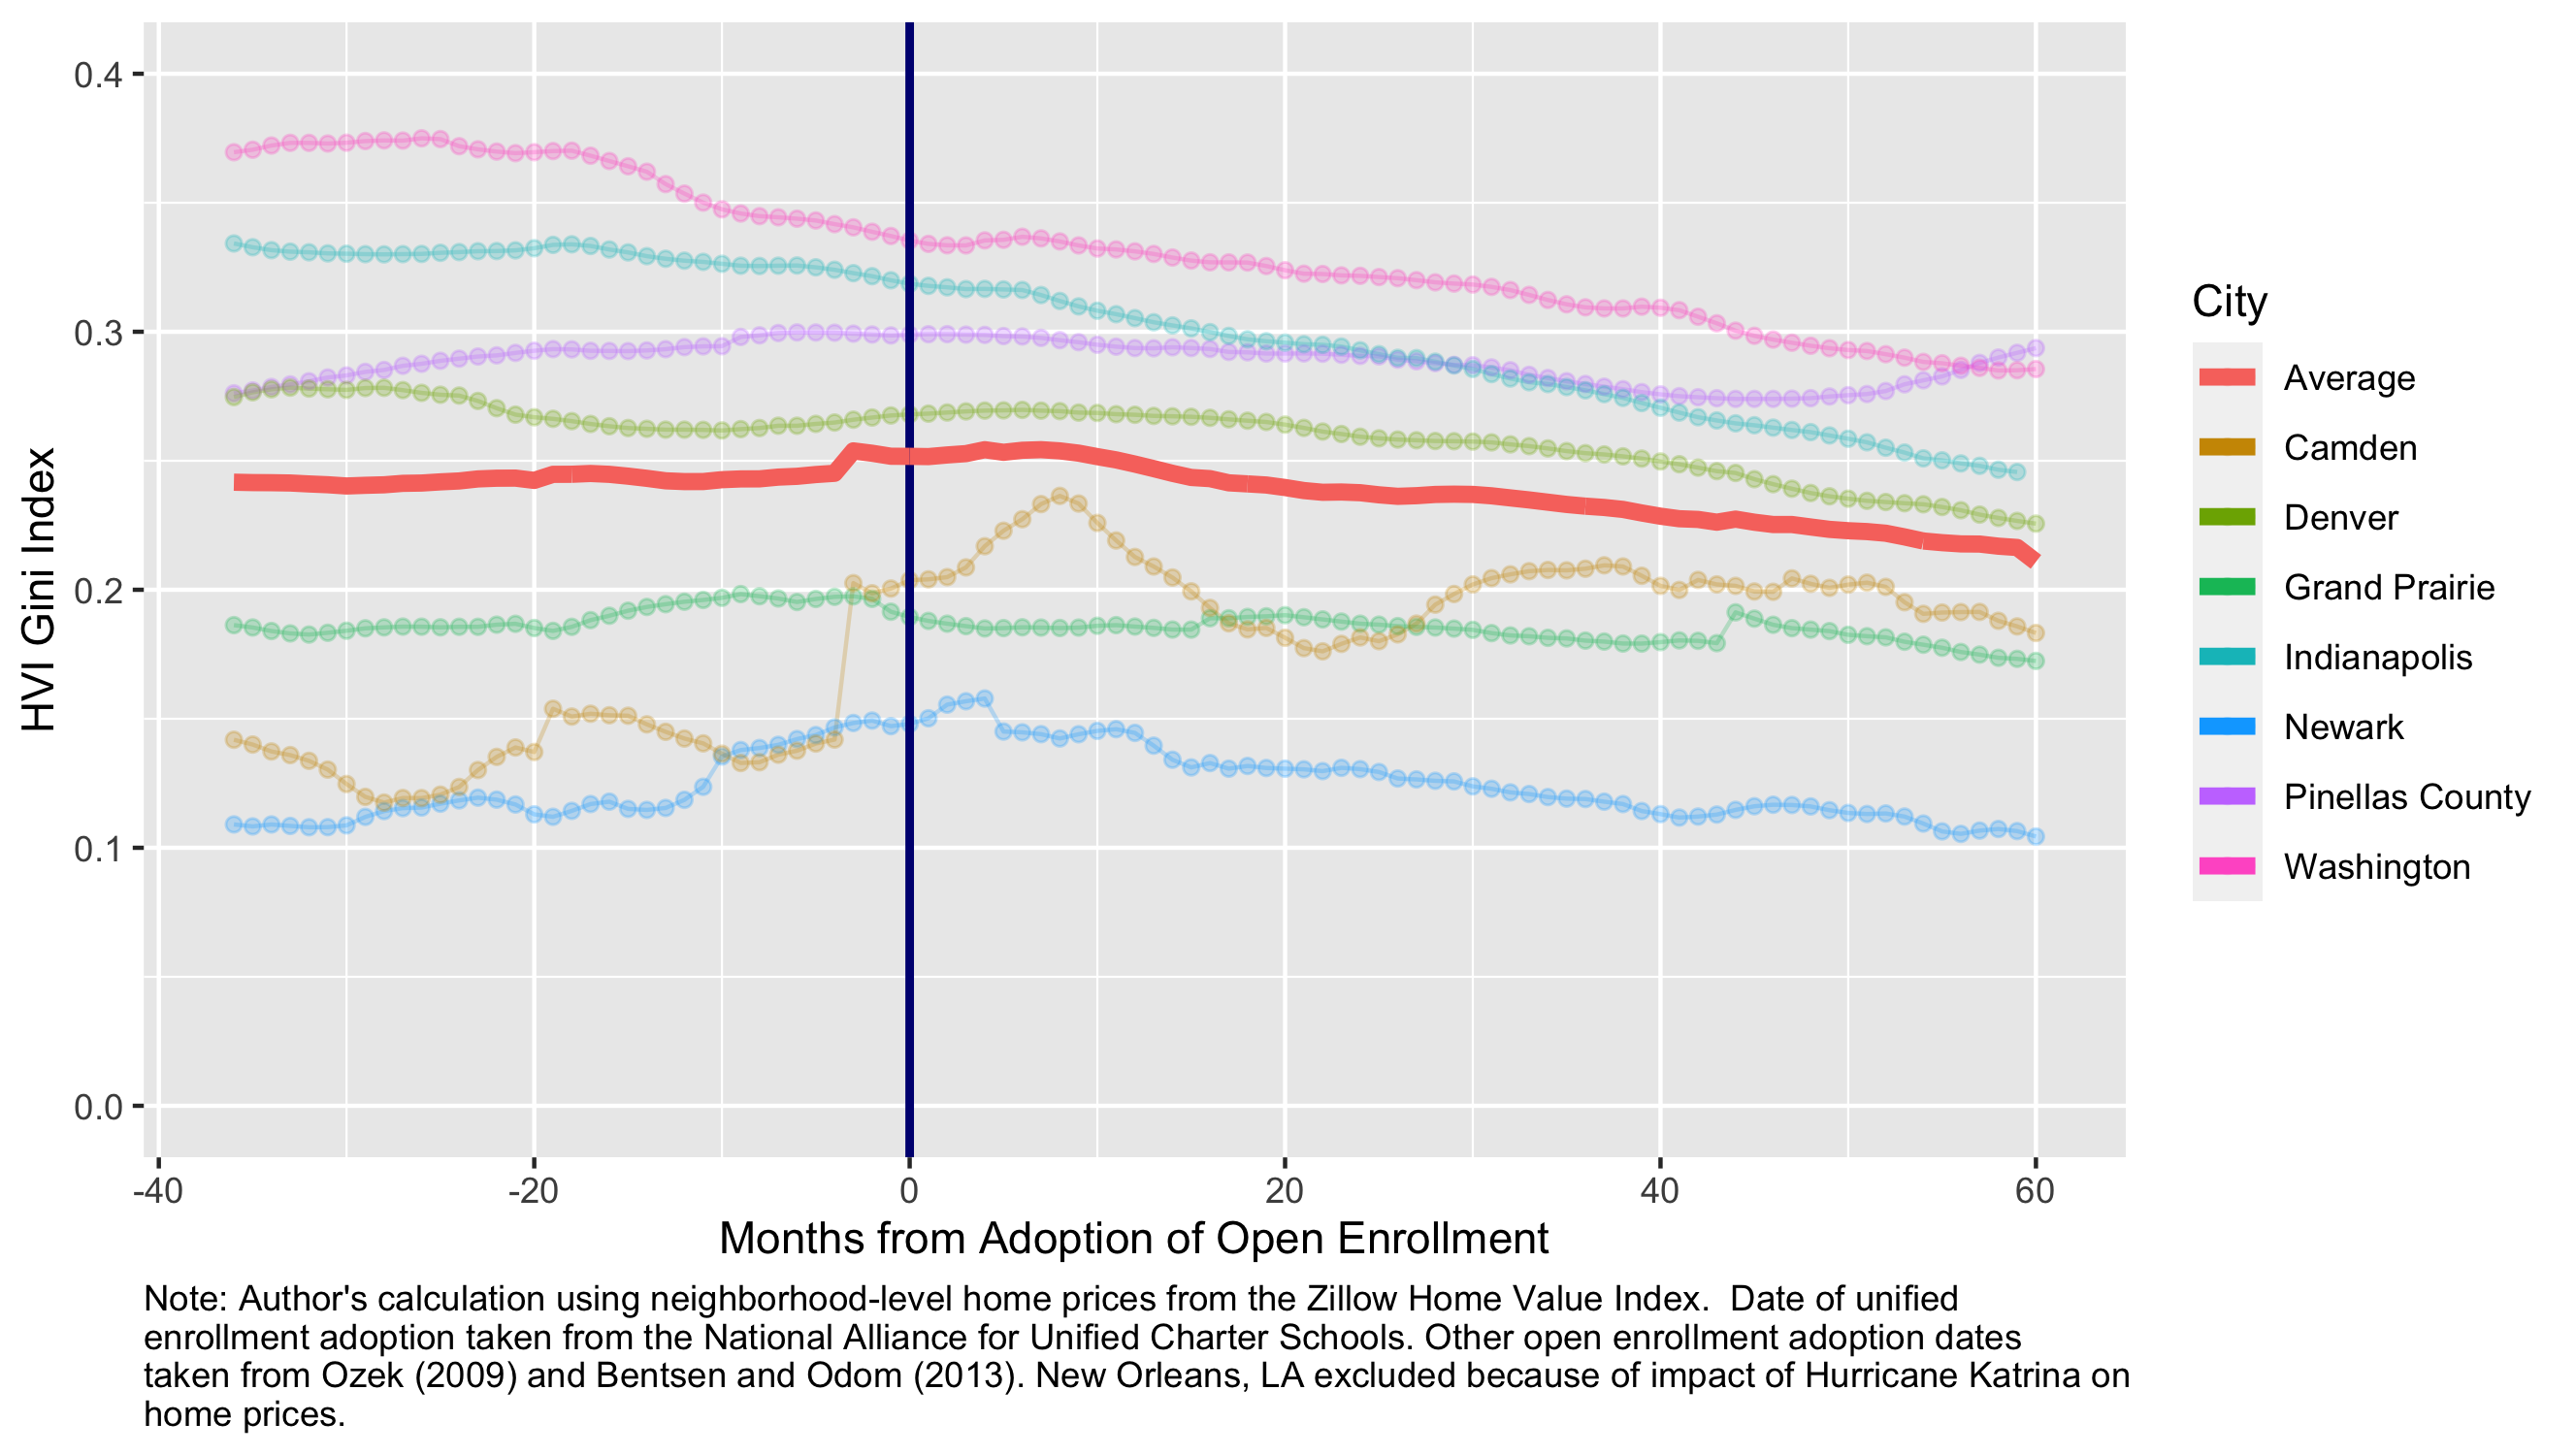
\includegraphics[width=0.9\textwidth]{figures/monthly_gini.png}
\hyperlink{giniback}{\beamerbutton{Back}}
\end{frame}

\begin{frame}{Adopters of Intradistrict Open Enrollment}
\label{sumstats}
% summary statistics table
\begin{table}[h] \centering 
\renewcommand{\arraystretch}{1.25}
    %\caption{Student Summary Statistics} 
    \label{sumstats} 
  \scriptsize 
  \begin{tabular}{@{\extracolsep{5pt}}lcccccccc} 
  \\[-1.8ex]\hline 
  \hline \\[-1.8ex] 
  \textit{Districts} & Adoption & State & \# Schools & \# Students & \$/Student & STR & \% URM & \% FRPL \\ 
  \hline \\[-1.8ex] 
  Camden & 2016 & NJ & 20 & 7,638 & \$28,845 & 9.5 & 98.6\% & 51.3\% \\
  Denver & 2011 & CO & 206 & 92,039 & \$12,639 & 15.0 & 70.1\% & 55.9\% \\
  Grand Prairie & 2012 & TX & 41 & 29,200 & \$9,984 & 15.4 & 86.2\% & 67.5 \% \\
  Indianapolis & 2018 & IN & 59 & 26,410 & \$12,452 & 14.0 & 73.9\% & 63.9\% \\ 
  Newark & 2014 & NJ & 64 & 40,448 & \$20,566 & 14.5 & 91.1\% & 61.1 \% \\  
  Pinellas County & 2003 & FL & 157 & 100,948 & \$9,952 & 13.4 & 40.9\% & 44.7\% \\  
  Washington & 2014 & DC & 113 & 49,065 & \$22,406 & 12.1 & 81.5\% & -- \\  
  \midrule
  US Average & -- & -- & 5.4 & 2,859 & \$17,050 & 15.6 & 35.0\% & 39.7\% \\  
  \midrule \midrule
  \multicolumn{9}{l}{\parbox{15cm}{Note: STR denotes student-teacher ratio. Aside from adoption dates, all school district data is from the 2018-2019 NCES CCD, the last year in which district financial data is available. School districts reporting 0 enrollment and non-traditional districts (i.e. charters) are dropped from the sample when calculating national averages.}}
  \end{tabular}
  \end{table} 
  \hyperlink{giniback}{\beamerbutton{Back}}
\end{frame}

\begin{frame}{Data}
\label{data} 
\begin{wideitemize}
\item Today
\begin{wideitemize}
\item \textbf{Aggregated Home Prices:} FHFA HPI, Zillow HVI
\item \textbf{Neighborhood Demographics:} ACS, Census
\item \textbf{School District Characteristics:} NCES CCD
\item \textbf{Open Enrollment Adoption Dates:} NAPCS
\end{wideitemize}
\item Future
\begin{wideitemize}
  \item \textbf{Home Prices and Characteristics:} CoreLogic
  \item \textbf{School Attendance Zone Boundaries:} SABINS
\end{wideitemize}
\end{wideitemize}
\hyperlink{databack}{\beamerbutton{Back}}
\end{frame}

\begin{frame}{District Diff-in-Diff: Gini Index (Mean = 22.4)}
\label{gini_did}
\begin{figure}
\centering
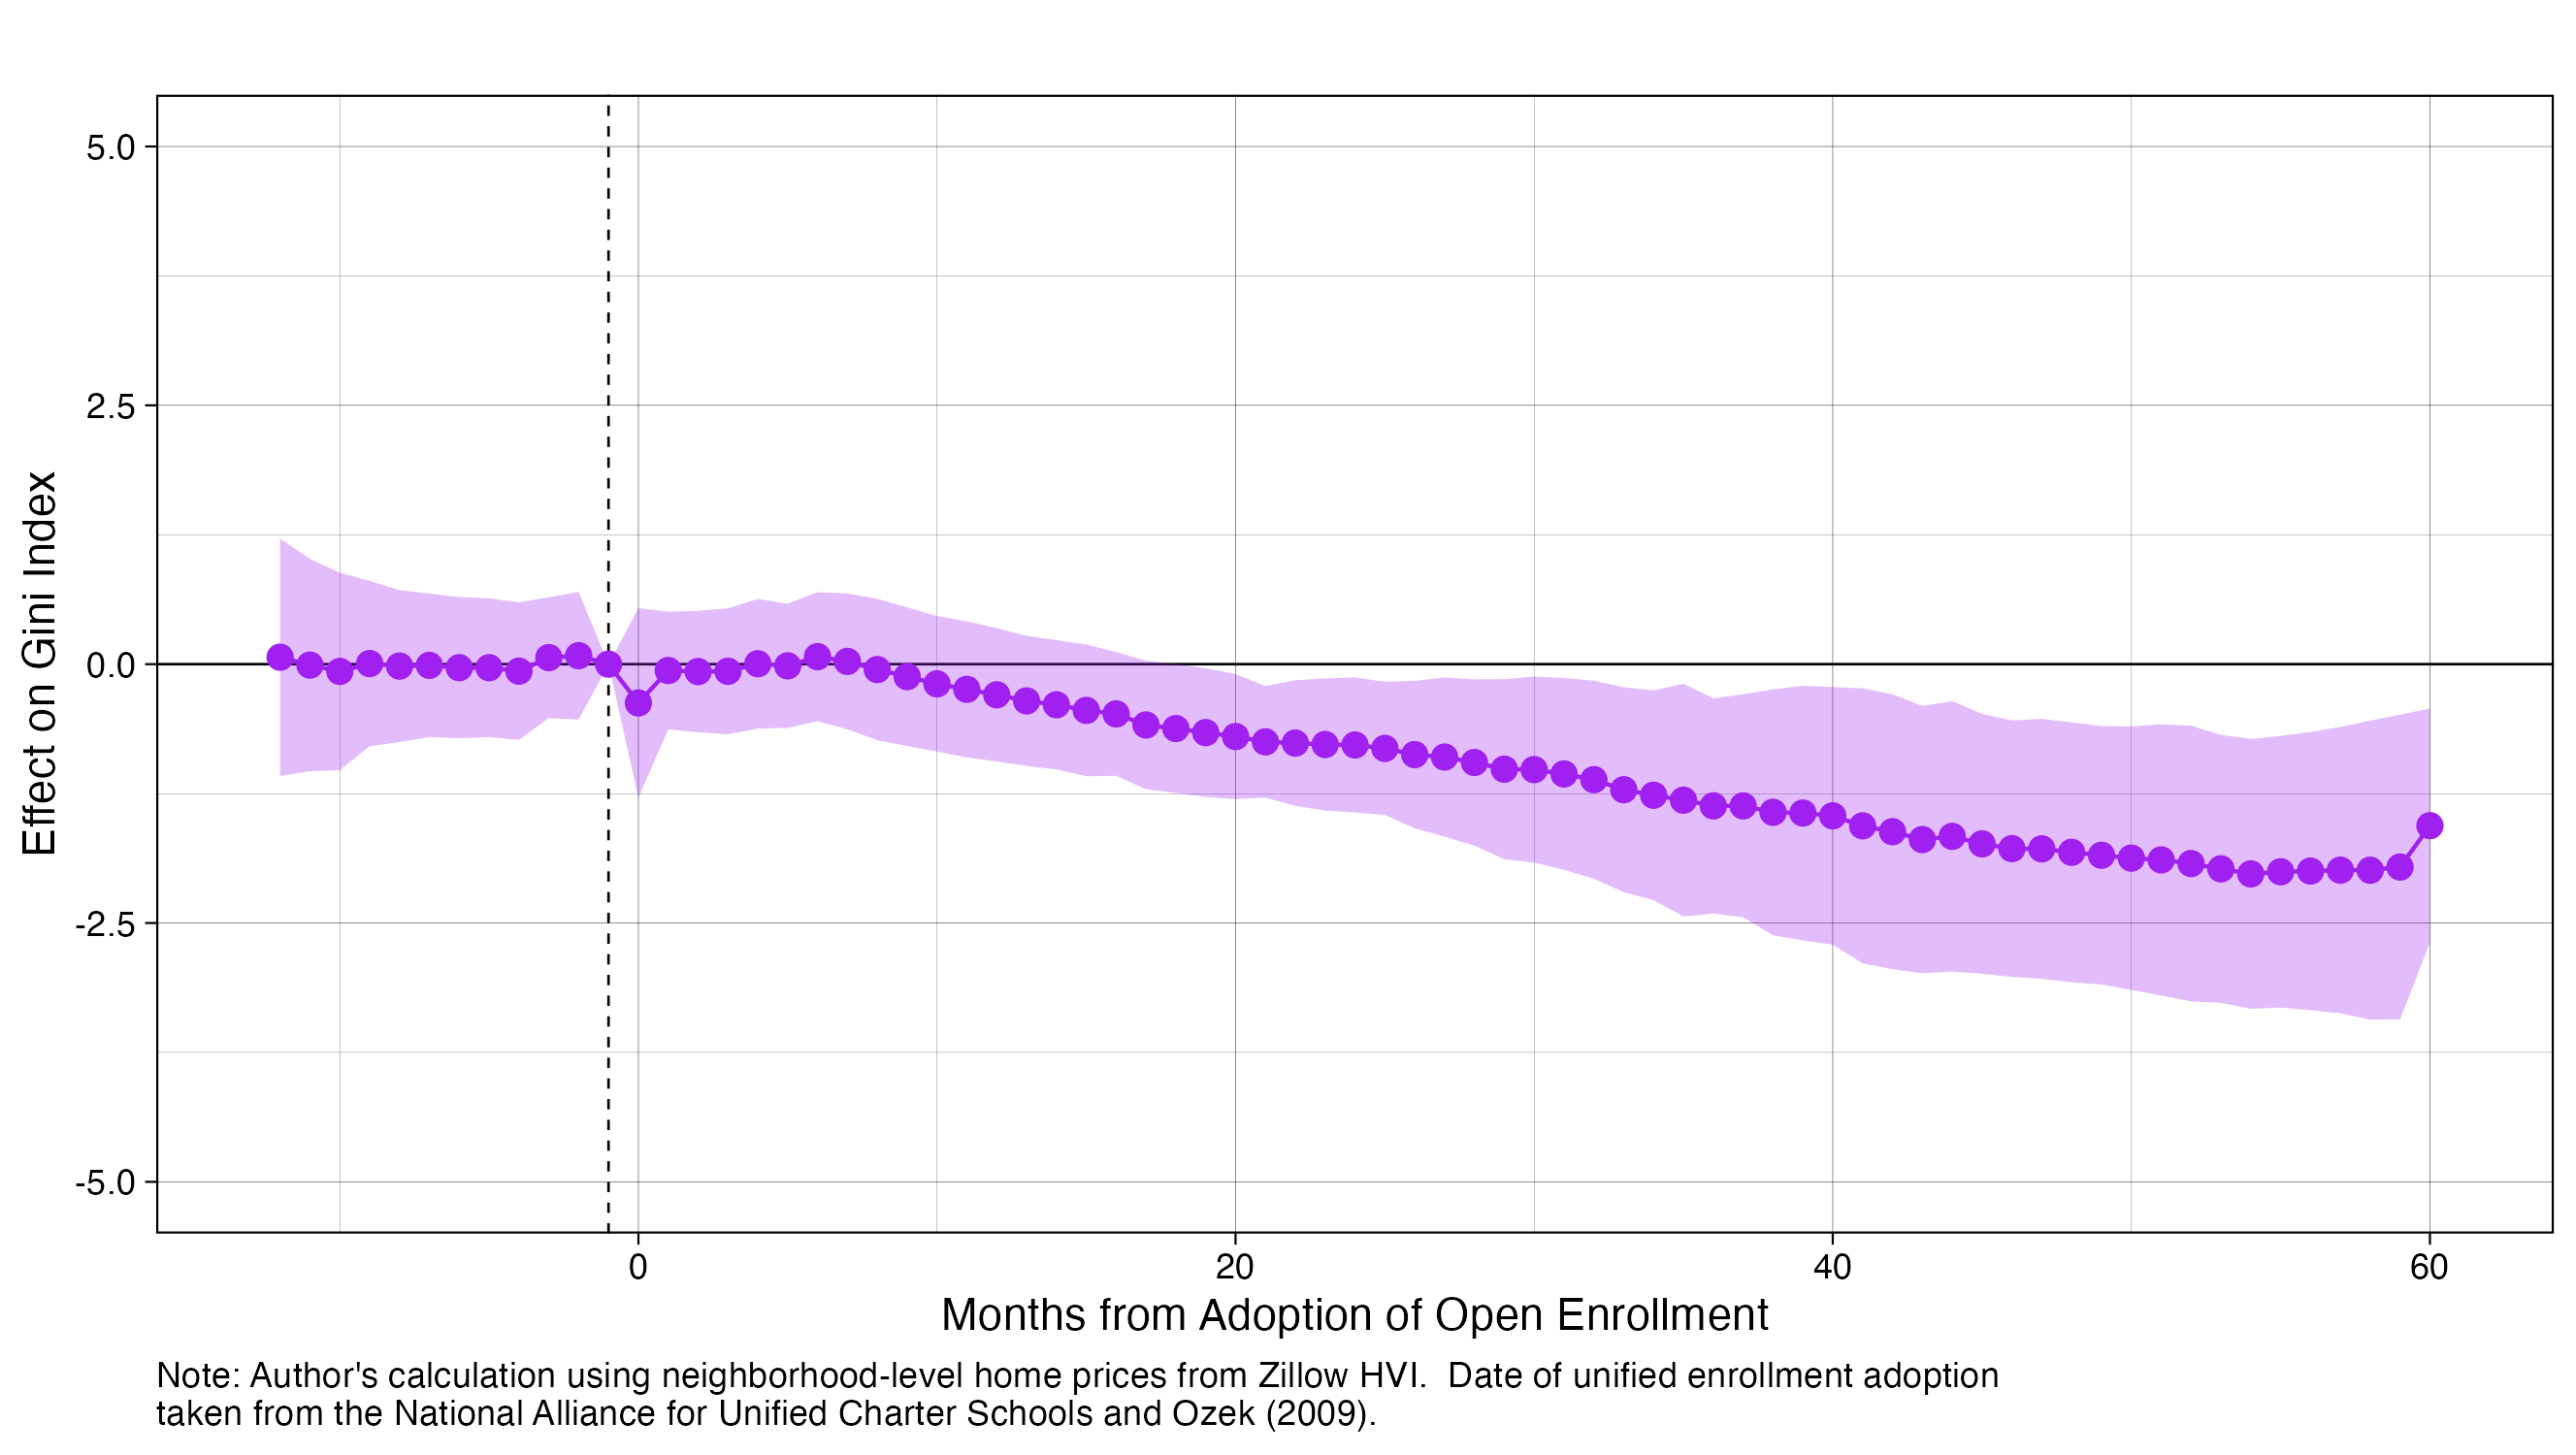
\includegraphics[width=0.8\textwidth]{figures/event_study_gini.png}
\end{figure}
\hyperlink{sd}{\beamerbutton{Back}}
\end{frame}

\begin{frame}{Stylized Model inspired by Avery and Pathak (2021)}
\label{details}
\begin{wideitemize}
\item \textbf{Details of Model}
\begin{enumerate}
\item Neighborhood school quality $q_n = E[x|x \text{ attends school }n]$
\item Competitive neighborhood home pricing rule $p(q_n)$
\item Utility from neighborhood with school quality $q$ 
\begin{equation*} u(x,q) = v(x,q) - p(q) - \textcolor{red}{C}\cdot \mathbf{1}\{ \text{Leave District}\}
\end{equation*} where $v(x,q)$ is supermodular. Notice that
\[\text{FOC of type $q$ household} \implies p(q) = \int_0^q \frac{\partial v(z,z)}{\partial q}dz\]
\end{enumerate}
\end{wideitemize}
\hyperlink{detailsback}{\beamerbutton{Back}}
\end{frame}

\begin{frame}{Stylized Model inspired by Avery and Pathak (2021)}
\label{location}
\begin{wideitemize}
\item \textbf{Household Location Decision}
\begin{enumerate}
\item Given $q_n$ and $p(q_n)$, select \textcolor{green}{within-district} neighborhood $n \in \{1,2\}$ that maximizes $u(x,q_n)$. Call this maximized value $D(x)$ and the neighborhood maximizer $n^*$
\item Select \textcolor{red}{out-of-district} school quality $q$ that maximizes $u(x,q)$. Under competitive pricing and supermodular $v(x,q)$, always choose $q=x$. Call this maximized value $O(x)$
\item Leave district if $O(x) > D(x)$. Otherwise, move to preferred neighborhood in district
\end{enumerate}
\end{wideitemize}
\hyperlink{detailsback}{\beamerbutton{Back}}
\end{frame}

\begin{frame}{Stylized Model inspired by Avery and Pathak (2021)}
\label{example}
\begin{wideitemize}
\item \textbf{Simple Numerical Example}
\begin{enumerate}
\item Suppose $x \sim U(0,1)$ and $v = x \cdot q$. The latter implies $p(q) = \frac{q^2}{2}$
\item $D(x) = x \cdot q_{n^*} - \frac{q_{n^*}^2}{2}$
\item $O(x) = x^2 - \frac{x^2}{2} - \textcolor{red}{C}$
\item Exit when $O(x) > D(x) \iff \frac{(x-q_{n^*})^2}{2} > \textcolor{red}{C} $
\end{enumerate}
\end{wideitemize}
\hyperlink{detailsback}{\beamerbutton{Back}}
\end{frame}

\end{document}